\chapter{Разработка метода, способного оперировать действиями различного масштаба, устойчивого к оптическим шумам, и его применение для настройки оптического интерферометра}\label{ch:ch2}

\section{Физические принципы работы и модель оптического интерферометра}\label{sec:ch2/sec1}

\subsection{Математическая модель интерференции света}\label{sec:ch2/sec1/subsec1}

Работа оптического интерферометра основана на принципе интерференции света --- физического процесса, при котором два когерентных световых пучка накладываются друг на друга и образуют в пространстве периодическую структуру, состоящую из минимумов и максимумов интенсивности, получившую название интерференционной картины. 

\begin{figure}[ht]
    \centerfloat{
        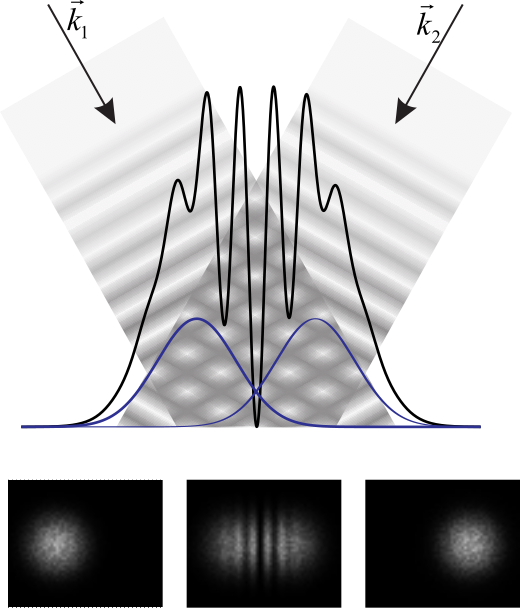
\includegraphics[scale=1.7]{images/interf_expl.png}
    }
    \caption{Одномерный срез интерференционной картины, полученный при неполном перекрытии двух когерентных лазерных лучей с волновыми векторами $k_1$ и $k_2$. Волновые фронты показаны с помощью градиента. Голубые линии показывают интенсивности индивидуальных лучей (не в масштабе). Черные линии соответствуют профилю интенсивности результирующей картины. Соответствующие двумерные изображения индивидуальных лучей и их интерференционной картины представлены внизу.}\label{fig:two_beam_interf}
\end{figure}

Интерференционная картина, получаемая при наложении двух когерентных лучей, изображена на рис. \ref{fig:two_beam_interf}. Для вычисления интерференционной картины опишем математическую модель интерференции. Рассмотрим световой пучок, распространяющийся вдоль оси $z$ в параксиальном приближении $k_z \gg k_x, k_y$, где волновой вектор $\vec{k}$ --- вектор, направление которого перпендикулярно фазовому фронту волны, а абсолютное значение равно волновому числу. Волновое число $k$ связано с длиной волны $\lambda$ соотношением:

\begin{equation*}
    k = \frac{2\pi}{\lambda}
\end{equation*}

Распределение амплитуды излучения будем описывать с помощью нормального распределения. Определим радиус пучка $r$ как расстояние от центра пучка, на котором напряженность электромагнитного поля падает в $e$ раз. 
Тогда распределение напряженности электромагнитного поля в каждом световом пучке $E(x, y, z)$ с плоским волновым фронтом и гауссовым профилем задается следующим выражением: 

\begin{equation}
    E(x,y,z) = \exp \left(-\frac{(x-x_0(z))^2+(y-y_0(z))^2}{r^2} \right) \cdot \exp \left(i k_xx+ik_yy+ik_zz\right),
\label{eq:Exyzt}
\end{equation}
где $(x,y,z)$ --- координатный вектор, $(x_0(z),y_0(z))$ --- положение центра пучка, $\vec{k}$ --- волновой вектор, $r$ --- радиус пучка. Уравнение \eqref{eq:Exyzt} не учитывает дифракционную расходимость пучка. 
Первый множитель в уравнении \eqref{eq:Exyzt} соответствует амплитуде электромагнитной волны $A(x,y,z)$, а второй --- фазе $\exp(i\phi(x,y,z))$. 
При сложении двух электромагнитных волн в точке $x, y, z$ итоговая напряженность поля будет равна сумме напряженностей отдельных волн: 

\begin{equation}
    E(x, y, z) = E_1(x, y, z) + E_2(x, y, z)
\label{eq:E1E2}
\end{equation}

Видимая интерференционная картина определяется распределением интенсивности света, которая равна квадрату модуля напряженности электромагнитного поля: 

\begin{equation}
    I(x, y, z) = |E(x, y, z)|^2 = E(x,y,z) \cdot E^*(x,y,z),
\label{eq:ie2}
\end{equation}
где $E^*$ --- комплексно-сопряженное значение напряженности электромагнитного поля. Таким образом, в соответствии с уравнениями \eqref{eq:Exyzt}, \eqref{eq:E1E2}, \eqref{eq:ie2}, интенсивность света в точке $x, y, z$ при сложении двух световых пучков определятся выражением: 

\begin{multline}
    I(x, y, z) = E_1E_1^* + E_2E_2^* + E_1E_2^* + E_2E_1^* = \\
    I_1(x,y,z) + I_2(x,y,z) + 2 \sqrt{I_1(x,y,z)I_2(x,y,z)}\cos(\Delta \phi),
\label{eq:interf}
\end{multline}
где $\Delta \phi = \phi_1 - \phi_2$ --- разность фаз двух волн. Из уравнения \eqref{eq:interf} следует, что в тех точках пространства, где две волны складываются синфазно ($\Delta \phi = 0$), интенсивность света максимальна $I = I_1 + I_2 + 2\sqrt{I_1I_2}$. В точках пространства, где волны складываются в противофазе ($\Delta \phi = \pi$), интенсивность света минимальна $I = I_1 + I_2 - 2\sqrt{I_1I_2}$.

\subsection{Математическая модель интерферометра Маха-Цендера}\label{sec:ch2/sec1/subsec2}

Интерферометры являются одними из основных инструментов в экспериментальной оптике и служат для прецизионного измерения разности фаз между двумя когерентными лучами.  Интерферометр Фабри-Перо\cite{fabry-perot1899} используется в оптической спектрометрии. Интерферометр Майкельсона является основной частью современных детекторов гравитационных волн LIGO и VIRGO \cite{LIGO, VIRGO}. Он также используется для измерения шероховатости поверхностей. Интерферометр Саньяка используется в современных навигационных системах. Интерферометр Маха-Цендера является основным инструментом в современных экспериментах в квантовой оптике \cite{Sarkar2006, Sychev2017}. 

\begin{figure}[ht]
\centerfloat{
    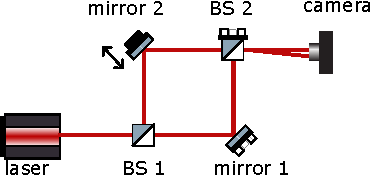
\includegraphics[scale=2.0]{images/MZI_expl.pdf}
}
\caption{Принципиальная схема работы интерферометра Маха-Цендера.}
\label{fig:MZI}
\end{figure}

В рамках данной работы рассматривалась настройка оптического интерферометра Маха-Цендера методами машинного обучения с подкреплением. Схема работы интерферометра Маха-Цендера изображена на рис. \ref{fig:MZI}. На схеме лазерный луч после прохождения светоделителя $BS\ 1$ разделяется на два луча. Верхний луч проходит через зеркало $mirror\ 2$ и светоделитель $BS\ 2$ и попадает на камеру. Нижний луч проходит через светоделитель $BS\ 1$ и зеркало $mirror\ 1$. Для настройки интерферометра необходимо точно совместить два луча как по положению, так и по направлению на камере. Регулировка нижнего луча производится с помощью зеркала $mirror\ 1$ и светоделителя $BS\ 2$. Верхний луч является неподвижным. Настройка интерферометра представляет собой итеративный процесс, в котором человек, ориентируясь на интерференционную картину, получаемую на камере, подстраивает положение зеркала $mirror\ 1$ и светоделителя $BS\ 2$, чтобы добиться идеального совпадения лучей. Для визуализации разности фаз между двумя плечами интерферометра зеркало $mirror\ 2$ совершает колебательные движения на расстояние порядка длины волны $\lambda$, благодаря чему фаза верхнего луча изменяется в интервале $\phi \in [0, 2\pi)$. Настройка интерферометра представляет собой трудоемкий процесс, осложненный тем, что и зеркало $mirror\ 1$, и светоделитель $BS\ 2$ меняют одновременно как положение луча на камере, так и угол между лучами. 

\begin{figure}[ht]
\centerfloat{
    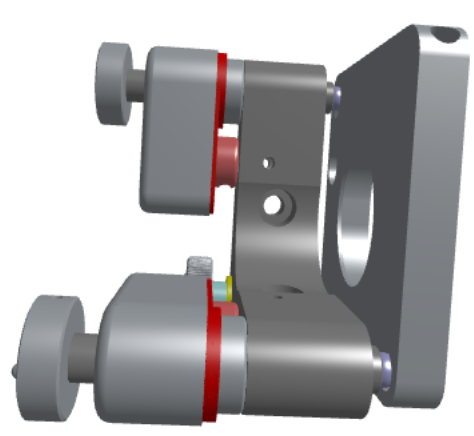
\includegraphics[scale=0.3]{images/mirror_mount.png}
}
\caption{3D модель крепления оптического зеркала использованного в работе \cite{newport_mirror}}
\label{fig:mirror}
\end{figure}

На рис. \ref{fig:mirror} показана 3D модель крепления оптического зеркала, использованная в работе для регулировки положения зеркала $mirror\ 1$ и светоделителя $BS\ 2$. Крепление оборудовано двумя микрометрическими винтами, которые могут как управляться с помощью встроенных пьезо двигателей, так и вращаться вручную. Каждый из винтов поворачивает зеркало вокруг одной из двух перпендикулярных осей. Направление вектора нормали зеркала $\vec{n}$ зависит от положений винтов $x, y$ в приближении малых углов следующим образом: 

\begin{equation}
    \vec{n} = \begin{pmatrix}
        x\\ 
        y\\ 
        \sqrt{1 - x^2 - y^2}
    \end{pmatrix}
\end{equation}


Для вычисления интерференционной картины по формуле \eqref{eq:interf} необходимо знать положение центров лучей и фазы, с которыми они интерферируют в каждом из пикселей камеры. Введем систему координат с центром в камере, как показано на рис. \ref{fig:MZI_coordis}. Предполагаем, что верхний луч распространяется точно вдоль оси  $z$. Таким образом, для него $x_0\equiv y_0\equiv k_x\equiv k_y\equiv 0$. Для нахождения центра и направления нижнего луча будем производить трассировку  луча через систему зеркал. 

\begin{figure}[ht]
\centerfloat{
    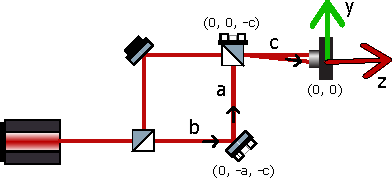
\includegraphics[scale=2.0]{images/MZI_matmodel.pdf}
}
\caption{Задание системы координат для интерферометра Маха-Цендера.}
\label{fig:MZI_coordis}
\end{figure}

При трассировке во время отражения луча от зеркала вычисляется точка пересечения луча с плоскостью зеркала и угол между направлением распространения луча и нормалью зеркала. Луч вращается относительно оси, перпендикулярной плоскости, образованной вектором нормали зеркала и  направлением распространения луча. Величина угла поворота определяется из закона отражения. Листинг функции трассировки приведен в приложении \ref{lst:beam_trace}.


\subsection{Видность интерференционной картины}\label{sec:ch2/sec1/subsec3}

Интенсивность интерференционной картины, получаемой при наложении двух лучей в плоскости камеры ($z=0$), задается выражением:

\begin{equation}
    I(x,y,t)=|E_1(x,y,0)+E_2(x,y,0)e^{i\phi_{\mathrm{piezo}}(t)}|^2,
\label{eq:I_def}
\end{equation}
где $\phi_{\mathrm{piezo}}(t)$ фазовый сдвиг, получаемый из-за движения пьезо зеркала. Таким образом, разность фаз $\Delta \phi$ в уравнении \eqref{eq:interf} за один проход пьезо зеркала в каждой точке $(x, y)$ пробегает интервал от $0$ до $2\pi$. Суммарной интенсивностью интерференционной картины называется величина: 

\begin{equation}
    I_{\mathrm{tot}}(t) = \iint_{-\infty}^{+\infty} I(x, y, t) {\mathrm{d}}x{\mathrm{d}}y
\end{equation}

Периодическое движение пьезо зеркала приводит к периодическому изменению суммарной интенсивности. Пример изменения интенсивности интерференционной картины показан на рис. \ref{fig:intens_plot}.

\begin{figure}[ht]
\centerfloat{
    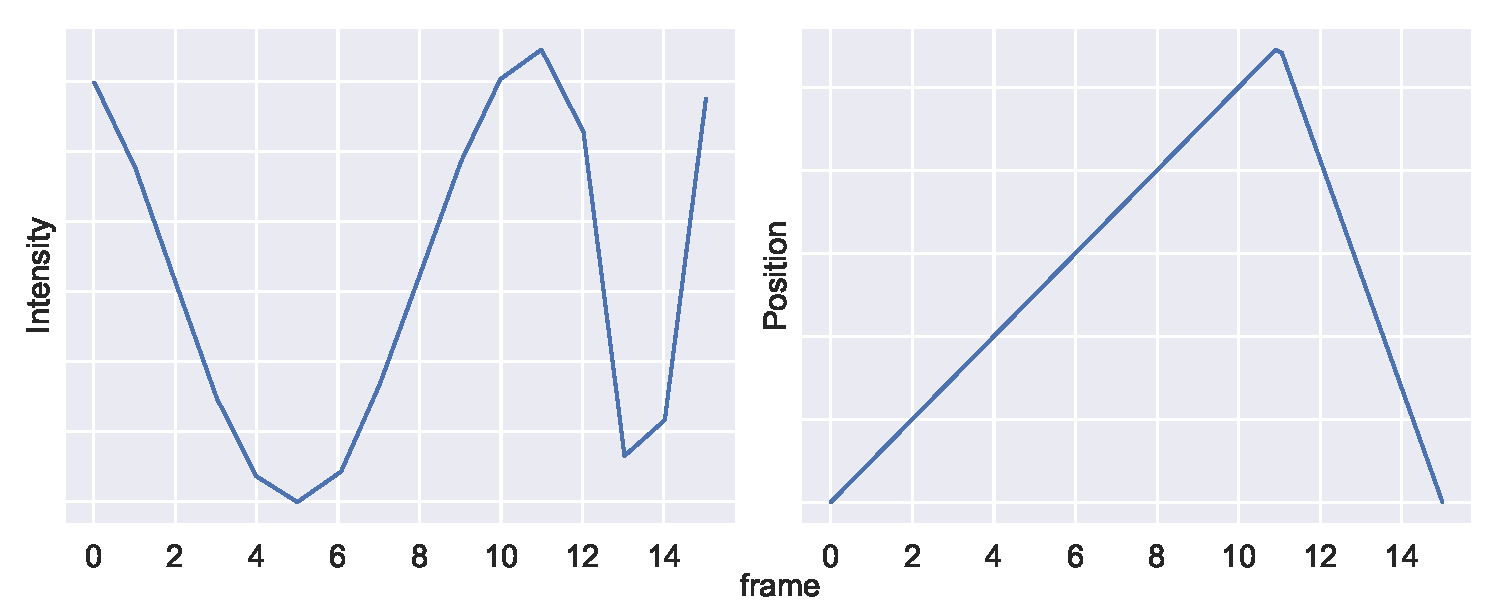
\includegraphics[scale=0.7]{images/intens_plot.pdf}
}
\caption{График изменения интенсивности (слева) и график движения пьезо зеркала (справа) от номера кадра (frame).}
\label{fig:intens_plot}
\end{figure}

Основным критерием качества настройки интерферометра является видность интерференционной картины: 

\begin{equation}
    V = \frac{            
        \max_{t}(I_{\mathrm{tot}}) - \min_t(I_{\mathrm{tot}})}
        {\max_{t}(I_{\mathrm{tot}}) + \min_t(I_{\mathrm{tot}})}
    \label{eq:visib}
\end{equation}

Видность интерференционной картины вычисляется с помощью минимума $\min_t(I_{\mathrm{tot}})$ и максимума $\max_t(I_{\mathrm{tot}})$ суммарной интенсивности света на камере. Максимум и минимум вычисляются за один полный период прохода пьезо зеркала. По определению, видность является действительным числом и находится в интервале $V \in [0, 1]$. Примеры интерференционных картин приведены на рис.~\ref{fig:visib_expl}. Для полностью настроенного интерферометра [рис.~\ref{fig:visib_expl}(a)], $\min_t(I_{\mathrm{tot}})=0$. Таким образом, видность $V=1$. Для полностью расстроенного интерферометра [рис.~\ref{fig:visib_expl}(c)], $\min_t(I_{\mathrm{tot}})\approx\max_t(I_{\mathrm{tot}})$. Таким образом, видность $V\approx 0$.

\begin{figure}[ht]
\centerfloat{
    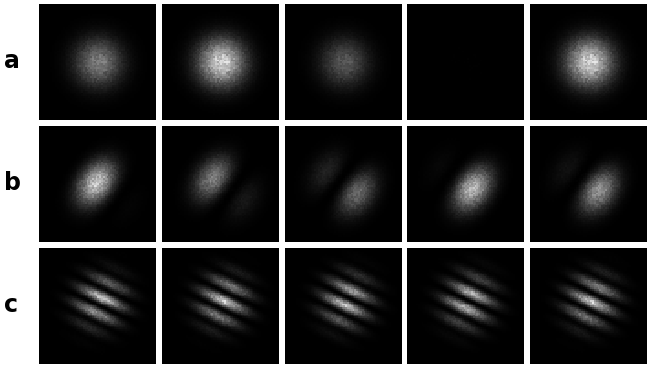
\includegraphics[scale=0.7]{images/visib_expl.png}
}
\caption{Примеры интерференционных картин, полученные в симуляции. (a) Полностью настроенный интерферометр. Видность = 1. (b) Слабо расстроенный интерферометр. Видность = 0.3. (c) Сильно расстроенный интерферометр. Видность =
0.0026. Изображения слева на право соответствуют различной разности фаз [$\phi_{\mathrm{piezo}}(t)$] между двумя плечами интерферометра из-за движения пьезо зеркала.}
\label{fig:visib_expl}
\end{figure}


Из уравнений~\eqref{eq:Exyzt} и \eqref{eq:visib}, получим точное выражение для видности интерференционной картины:

\begin{equation}
    V = \exp\left(- \frac{x_0^2 + y_0^2}{2 r^2}\right)  \exp\left[- \frac{(k_x^2 + k_y^2) r^2}{8}\right],
    \label{eq:visib_rot}
\end{equation}
где $x_0$ и $y_0$ --- координаты центра нижнего луча на камере, $k_x$ и $k_y$ --- компоненты волнового вектора нижнего луча. Вывод уравнения \eqref{eq:visib_rot} приведен в приложении \ref{app:B1}.

\subsection{Математическая модель интерферометра Маха-Цендера с линзами}\label{sec:ch2/sec1/subsec4}

Интерферометр Маха-Цендера, показанный на рис.~\ref{fig:MZI}, позволяет управлять положением луча на камере и его направлением. Однако он не позволяет управлять его волновым фронтом. Для этого, как показано на рис.~\ref{fig:MZI_expl_lenses}, в нижнее плечо интерферометра добавляют две собирающие линзы, установленные по схеме телескопа: расстояние между линзами в настроенном состоянии равно сумме из фокусных расстояний. Данная постановка более полно отражает задачи, возникающие в экспериментальной оптике. Во многих приложениях требуется добиться точного пространственного совпадения в распределениях электромагнитных полей лазерного пучка и мод резонатора или волновода. К таким приложениям относятся: 

\begin{itemize}
    \item Заведение лазерного пучка в оптоволокно.
    \item Заведение лазерного пучка в пассивный резонатор, который будет действовать в качестве пространственного или спектрального фильтра.
    \item Для работы мощного лазера с низкими шумами интенсивности и фазы применяется метод injection locking. В котором производится подача света из вспомогательного лазера с этой частотой в резонатор основного лазера. При этом необходимо добиться точного совпадения мод основного и вспомогательного лазеров.
\end{itemize}

При этом необходимо совпадение не только пространственных профилей интенсивности, но и фазовых.

\begin{figure}[ht]
\centerfloat{
    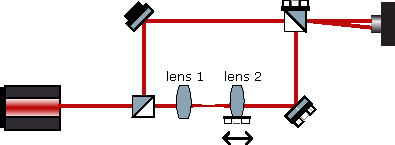
\includegraphics[scale=2.0]{images/MZI_expl_lenses.pdf}
}
\caption{Схема интерферометра Маха-Цендера с линзами.}
\label{fig:MZI_expl_lenses}
\end{figure}

В интерферометре, показанном на рис.~\ref{fig:MZI_expl_lenses}, помимо зеркала $mirror\ 1$ и светоделителя $BS\ 2$, настраивать еще нужно положение линзы $lens\ 2$. Положение линзы $lens\ 2$ регулируется с помощью подвижки, изображенной на рис.~\ref{fig:lense_mount}. 

\begin{figure}[ht]
\centerfloat{
    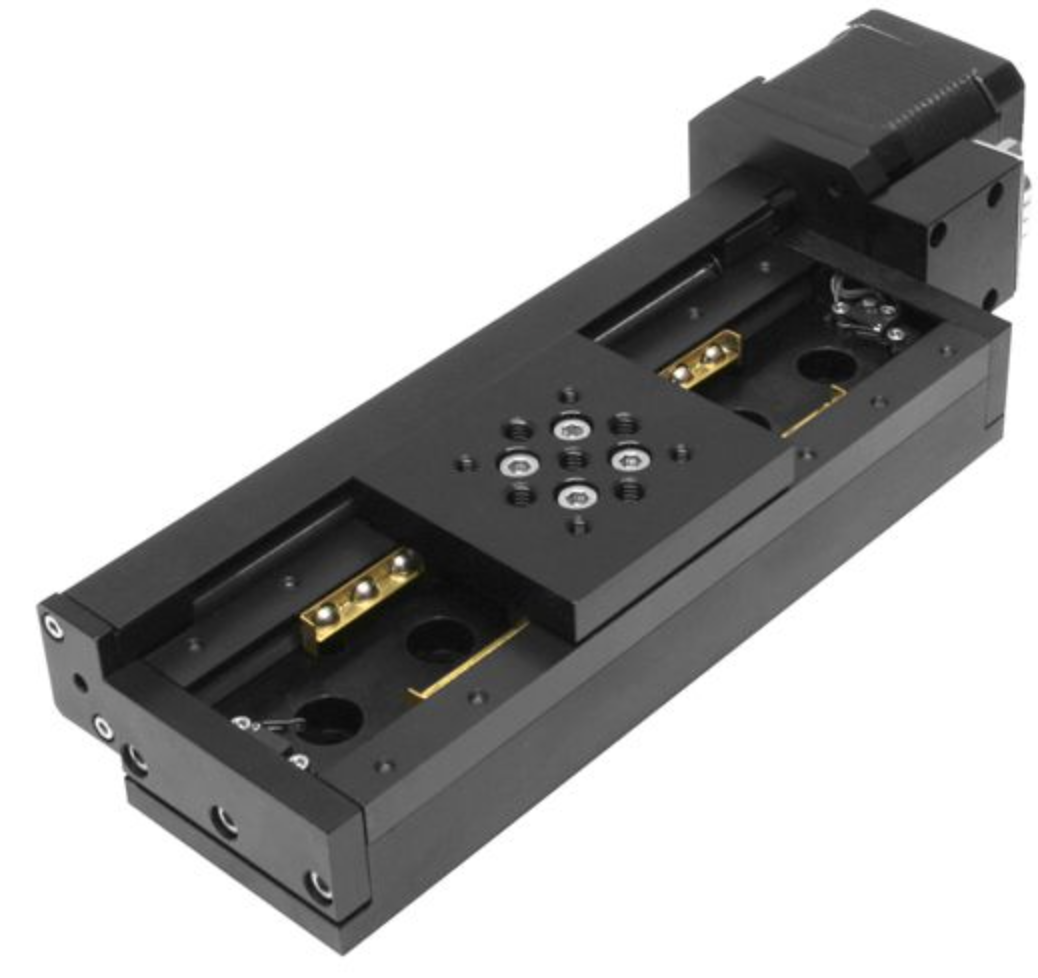
\includegraphics[scale=0.3]{images/lense_mount.png}
}
\caption{Подвижка регулирующая положение линзы 2 в эксперименте \cite{standa_stage}.}
\label{fig:lense_mount}
\end{figure}

Лазерные пучки в верхнем и нижнем плечах интерферометра описываются гауссовым поперечным профилем. Напряженность поля в точке с координатами $(x,y,z)$ задается следующим образом: 

\begin{subequations}\label{beams}
\begin{equation}
    E_u=\exp \left(-\frac{x^{2}+y^{2}}{r_u^{2}}\right) \cdot \exp \left(-i\left(k_{z} z + \phi_{\mathrm{piezo}}(t)\right)\right)
    \label{eq:upper_beam}
\end{equation}
\begin{equation}
    \label{eq:lower_beam}
    \begin{split}
        E_l=\exp \left(-\frac{\left(x-x_{0}\right)^{2}+\left(y-y_{0}\right)^{2}}{r_l^{2}(z)}\right) \cdot
        \exp \left(-i\left(k_{x} x+k_{y} y+k_{z} z + k\frac{x^2+y^2}{2\rho^2_l(z)} z\right)\right)
    \end{split}
    \end{equation}
\end{subequations}

В уравнениях (\ref{eq:upper_beam}, \ref{eq:lower_beam}) индексы $u$ и $l$ соответствуют пучкам, распространяющимся по верхнему и нижнему плечам интерферометра соответственно, $(x_0, y_0)$ --- положение центра нижнего луча [верхний луч считается центрированным в $(x,y)=(0,0)$], $z$ --- направление распространения лучей, $r(z)$ --- радиус луча, $\rho(z)$ --- радиус кривизны волнового фронта, $(k_x,k_y,k_z)$ --- волновой вектор $k=\sqrt{k_x^2+k_y^2+k_z^2}=2\pi/\lambda$, $\phi_{\mathrm{piezo}}(t)$ --- фазовый сдвиг из-за движения пьезо зеркала. Также используется параксиальное приближение $k_z \gg k_x, k_y$. В отличие от уравнения \eqref{eq:Exyzt}, в уравнении \eqref{eq:lower_beam} волновой фронт уже не является плоским, а зависит от радиуса кривизны волнового фронта $\rho(z)$. Кроме того, появляется зависимость радиуса пучка от расстояния $r(z)$. 

Для моделирования параметров пучка после прохождения системы линз воспользуемся матричным методом \cite{gerrard2012introduction}. В этом методе световой луч характеризуется комплексно значным параметром $q$:

\begin{equation}
    \dfrac{1}{q} = \dfrac{1}{\rho} - \dfrac{i \lambda}{\pi r^2}   
\label{eq:q_param}
\end{equation}

Преобразования, происходящие с лучом при прохождении оптических элементов, описываются четырьмя параметрами $ABCD$: 

\begin{equation}
    q^{\prime}=\dfrac{A q+B}{C q+D}
\label{eq:q_prime}
\end{equation}

Параметры $ABCD$ могут быть записаны в виде матрицы. Для пустого пространства длины $d$ $ABCD$-матрица имеет вид: 

\begin{equation}
    \begin{bmatrix} A & B \\ C & D \end{bmatrix}=\begin{bmatrix} 1 & d \\ 0 & 1 \end{bmatrix}
\label{eq:abcd_free}
\end{equation}

Для линзы с фокусным расстоянием $f$ $ABCD$-матрица имеет вид: 

\begin{equation}
    \begin{bmatrix} A & B \\ C & D \end{bmatrix}=\begin{bmatrix} 1 & 0 \\ -1/f & 1 \end{bmatrix}
\label{eq:abcd_lens}
\end{equation}

$ABCD$ матрица системы, состоящей из оптических элементов $M_1^{ABCD}$, $M_2^{ABCD}$, $M_3^{ABCD}$, будет равна произведению матриц для отдельных элементов:

\begin{equation}
    M = M_3^{ABCD} \times M_2^{ABCD} \times M_1^{ABCD}
\label{eq:abcd_prod}
\end{equation}

Умножение матриц происходит в порядке, обратном к их геометрическому расположению. Таким образом, для нахождения параметров пучка после прохождения интерферометра, помимо трассировки луча, требуется еще вычислить его параметры с помощью $ABCD$-матриц. Листинг функции, вычисляющей параметры пучка, приведен в приложении \ref{lst:beam_propag}.

\subsection{Видность интерференционной картины в интерферометре Маха-Цендера с линзами}\label{sec:ch2/sec1/subsec5}

Для получения аналитической зависимости видности интерференционной картины в интерферометре Маха-Цендера с линзами нужно вычислить перпендикулярные профили пучков  (\ref{beams}) и рассчитать видность в соответствии с уравнениями \eqref{eq:I_def}, \eqref{eq:visib}. Итоговое выражение для видности интерференционной картины выглядит следующим образом:

\begin{equation}
\begin{split}
    V =\frac{4}{\left(n^{2}+1\right) r_{\mathrm{u}}^{2}} \frac{1}{c} \exp \left(-\left(x_{0}^{2}+y_{0}^{2}\right)\left(\frac{1}{r_{\mathrm{u}}^{2} n^{2}}-\frac{n^{2}+1}{n^{6} r_{\mathrm{u}}^{6} c^{2}}\right)\right) \times \\ \times \exp \left(-\frac{n^{2}+1}{4 c^{2} n^{2} r_{\mathrm{u}}^{2}}\left(k_{x}^{2}+k_{y}^{2}\right)\right) \exp \left(\frac{\frac{\pi}{\lambda \rho^{\prime}}}{n^{2} r_{\mathrm{u}}^{2} c^{2}}\left(x_{0} k_{x}+y_{0} k_{y}\right)\right),
\end{split}
\label{eq:visib_lense}
\end{equation}
где параметр $n=\dfrac{r_{\mathrm{l}}}{r_{\mathrm{u}}}$ и параметр $c^2 = (\dfrac{n^2 + 1}{n^2r^2_{\mathrm{u}}})^2$.

Можно показать, что в случае, когда линзы полностью настроены ($r_{\mathrm{u}} = r_{\mathrm{l}}$, $\rho^{\prime} = \rho = \infty$) выражение \eqref{eq:visib_lense} совпадает с формулой \eqref{eq:visib_rot}. Полный вывод формулы \eqref{eq:visib_lense} приведен в приложении \ref{app:B2}.

Примеры интерференционных картин, получаемые в интерферометре Маха-Цендера с линзами, приведены на рис.~\ref{fig:visib_lens_expl}. Закругленная форма интерференционных полос появляется в следствии интерференции пучков с различной расходимостью. Мы прикладываем ассиметричное пилообразное напряжение к пьезо зеркалу для наблюдения временной динамики интерференционных полос. Амплитуда движения пьезо зеркала соответствует разности фаз пучков порядка $2\pi$. Для расстроенного интерферометра, движение пьезо зеркала приводит к поперечному смещению интерференционных полос, как показано на рис. \ref{fig:visib_lens_expl}(b-d), что позволяет извлечь информацию о знаке угла между интерферирующими лучами. В случае, если интерферометр полностью настроен, интерференция будет выглядеть как мигающее пятно [рис. \ref{fig:visib_lens_expl}(a)].

\begin{figure}[ht]
\centerfloat{
    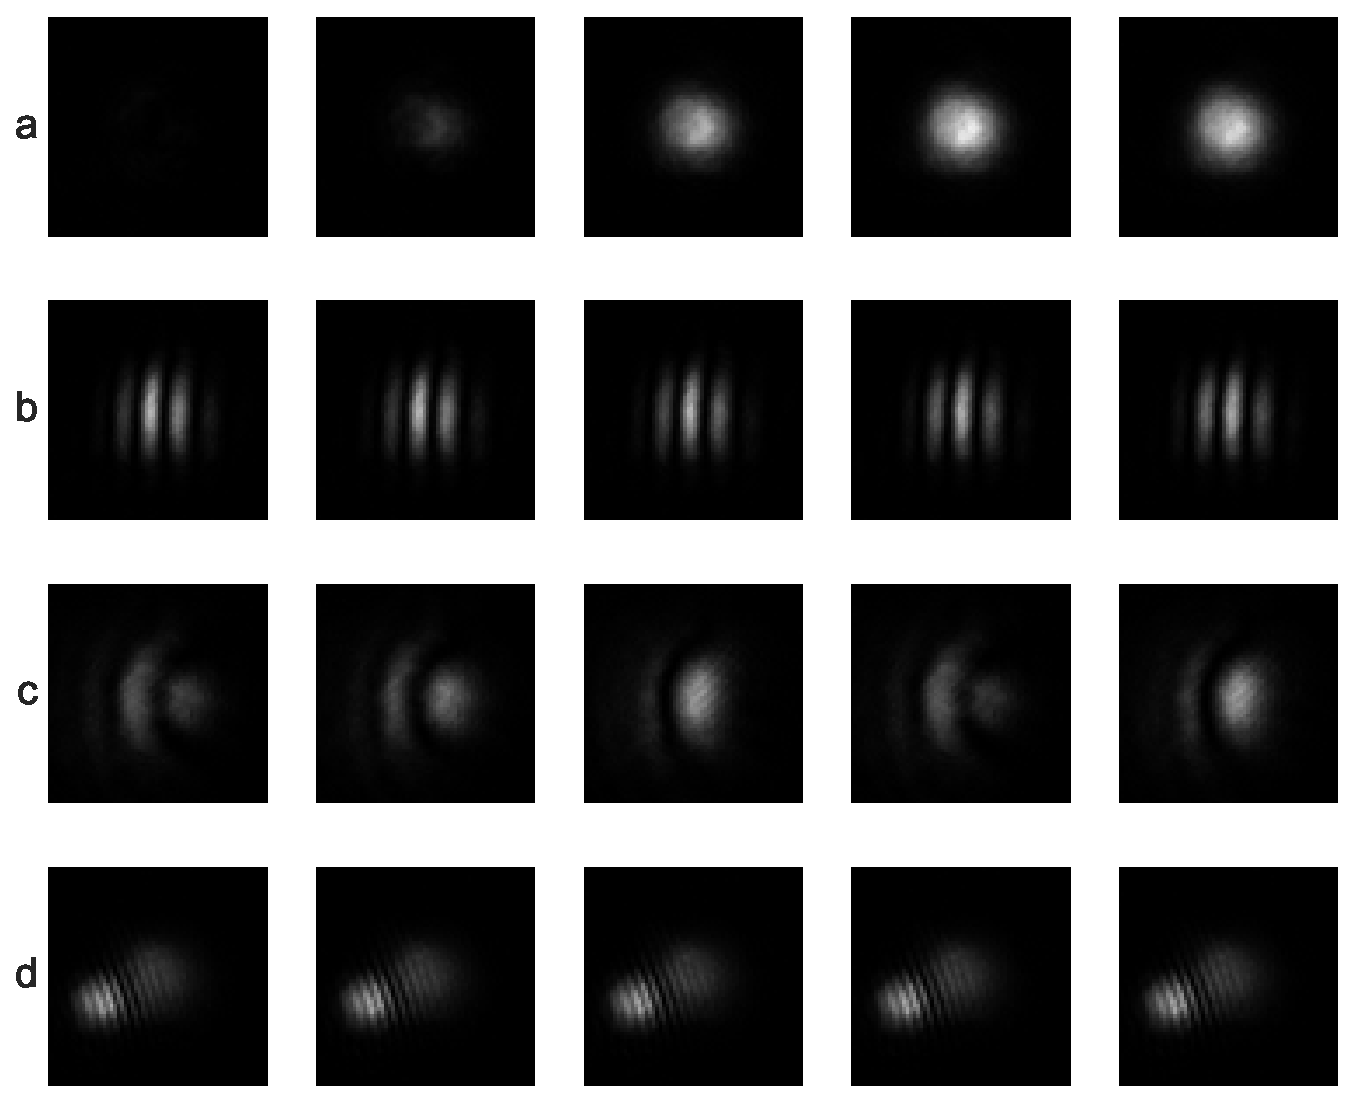
\includegraphics[scale=0.7]{images/Env_patterns.pdf}
}
\caption{Примеры интерференционных картин, полученные на интерферометре Маха-Цендера с линзами. (a) Пример интерференционных изображений при настроенном интерферометре. (b-d) Пример интерференционных изображений, полученных при расстроенном интерферометре. Изображения в каждом столбце соответствуют различным положениям пьезо зеркала.}
\label{fig:visib_lens_expl}
\end{figure}

\subsection{Численная модель интерферометра Маха-Цендера}\label{sec:ch2/sec1/subsec6}

При вычислении интерференционной картины трассировка центра пучка и вычисление его радиуса и кривизны волнового фронта производится согласно описанию в разделах: \ref{sec:ch2/sec1/subsec2}, \ref{sec:ch2/sec1/subsec4}. Основная вычислительная сложность состоит в нахождении изображения интерференционной картины согласно ур.~\eqref{eq:interf}. Изображение интерференционной картины будем рассчитывать на равномерной сетке размером $64\times64$ пикселя. За время одного прохода пьезо зеркала будем вычислять 16 интерференционных картин, соответствующих различным положениям пьезо зеркала $\phi_{\mathrm{piezo}}(t)$ взятым через одинаковые промежутки времени. 

Расчет интерференционной картины схематически показан на рис.~\ref{fig:wave_front_projection}. Алгоритм вычисления интерференционной картины \ref{alg:interf_img_calc} проецирует две волны на пиксели камеры и в каждом пикселе считает интенсивность результирующей волны согласно ур.~\eqref{eq:I_def}. В программе вычисление интерференционной картины реализовано на языке программирования C++ параллельно для каждого пикселя камеры. Листинг функции расчета интерференционной картины приведен в приложении \ref{lst:calcImage}. 

\begin{figure}[ht]
\centerfloat{
    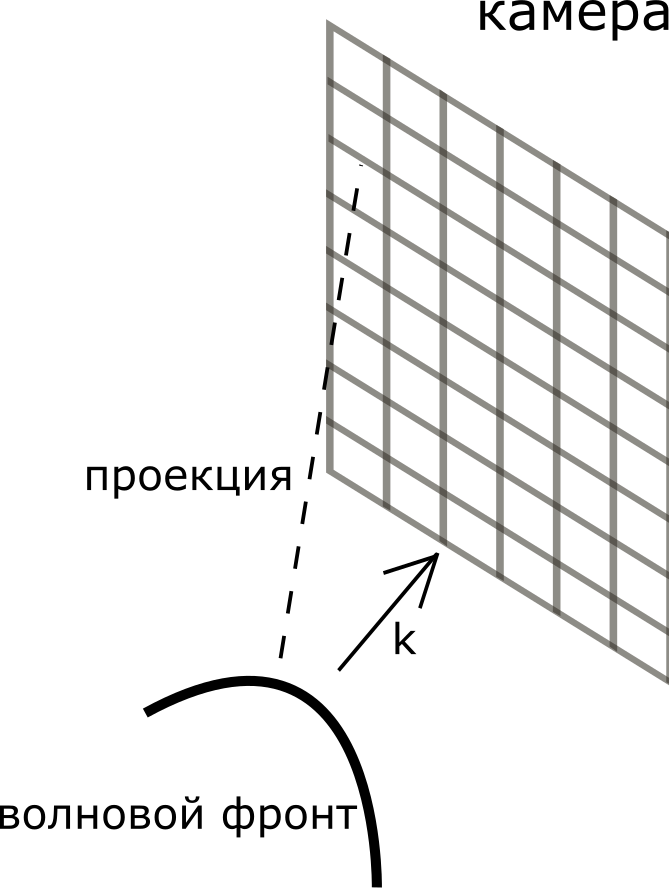
\includegraphics[scale=0.4]{images/wave_front_projection.png}
}
\caption{Вычисление интерференционной картины.}
\label{fig:wave_front_projection}
\end{figure}

\begin{algorithm}[ht]
	\SetAlgoLined
	\KwIn{$r_1, r_2$ - радиус $\rho_1, \rho_2$ - радиус кривизны, $(x,y)_1, (x,y)_2$ - координаты центра, $\vec{k}_1,\vec{k}_2$ - k-вектор, $N_{\mathrm{frames}}$ - число шагов по времени, $N_{\mathrm{pixels}}$ - число пикселей}
	\KwOut{image - 2d array}
	\ForEach{frame in $\{1...N_{\mathrm{frames}}\}$}{
	    \ForEach{pixel in $\{1...N_{\mathrm{pixels}}\}$}{
	        // найдем ортогональную проекцию пикселя на волновой фронт\;
            source1 = backTrack(pixel, $k_1$, $x_1$, $y_1$)\;
            source2 = backTrack(pixel, $k_2$, $x_2$, $y_2$)\;

	        // найдем расстояние пройденое лучом\;
	        dist1 = dist(pixel, source1)\; 
	        dist1 = dist(pixel, source2)\; 

	        // рассчитаем амплитуду и фазу волны\;
	        w1 = calcWave(dist1, source1, $\rho_1$)\;
	        w2 = calcWave(dist2, source2, $\rho_2$)\;

	        // рассчитаем интенcивность света\;
	        image[pixel] = intens(w1, w2)\;
	    }
	}
\caption{Алгоритм вычисления интерференционной картины}
\label{alg:interf_img_calc}
\end{algorithm}


\section{Настройка оптического интерферометра как задача машинного обучения с подкреплением}\label{sec:ch2/sect2}

Рассмотрим более детально процесс настройки оптического интерферометра Маха-Цендера. Настройка представляет собой итеративный процесс, в котором человек подстраивает положения зеркал и линз в зависимости от текущей интерференционной картины, наблюдаемой на камере. Отличительной особенностью настройки интерферометра является необходимость получить значение видности как можно ближе к $1$. Это приводит к тому, что по мере приближения видности к $1$ требуется совершать действия все меньшего размера. Несмотря на то, что истинное состояние интерферометра (положение зеркал и линз) для человека недоступно, информации, получаемой из видео потока (размер интерференционных полос, их ориентация, их направление движения) в целом достаточно, чтобы понять, в какую сторону и примерно на сколько следует повернуть управляющие элементы. Интерференционную картину можно рассматривать как отображение из $n$-мерного пространства состояний ($\mathcal{R}^4$ для интерферометра с двумя зеркалами, $\mathcal{R}^5$ для интерферометра с двумя зеркалами и одной подвижной линзой) в пространство наблюдений --- двумерных изображений. Данное отображение не является взаимно-однозначным, но благодаря учету временной динамики и итеративному процессу настройки возможно восстановить настроенное состояние. 


\subsection{Пространство состояний и действий и длительность эпизода}

В рамках данной работы будем рассматривать процесс настройки оптического интерферометра как марковский процесс принятия решений. 

\paragraph{Пространство наблюдений.}
В качестве наблюдений будем рассматривать последовательность из 16 интерференционных изображений $64\times64$ пикселя, полученных во время прямого и обратного прохода пьезо зеркала. Данный подход позволяет включить временную динамику интерференционной картины в состояние среды. Благодаря различной длительности прямого и обратного прохода пьезо зеркала временная динамика интерференционной картины содержит информацию о знаке угла между $\vec{k}$-векторами интерферирующих лучей. Абсолютное значение угла между лучами определяется шириной интерференционных полос. Чем уже полосы, тем больше угол.

\paragraph{Пространство действий.}
При настройке интерферометра действия являются непрерывными величинами, означающими величину поворота зеркал или сдвига линз. При настройке интерферометра вручную человек последовательно вращает управляющие элементы зеркал. При обучении RL агента ограничим суммарную величину поворота зеркал $\alpha_{\max}$ и максимальное смещение линзы $\Delta_{max}$. Значения $\alpha_{\max}$ и $\Delta_{max}$ указаны в таблицах: \ref{tab:MZI_params}, \ref{tab:MZI_lens_params}. Ограничение на поворот зеркал $\alpha_{\max}$ не позволяет агенту отклонить зеркала слишком сильно, так как при этом ширина интерференционных полос может стать меньше размера пикселя итогово изображения. В частности, расстояние между центрами лучей не превышает трех радиусов луча и количество интерференционных полос на изображении не превышает 15. Ограничение на смещение линзы $\Delta_{max}$ не позволяет агенту получить размер пучка на изображении меньше пикселя или больше размера матрицы камеры. В нашей работе рассмотрим две подхода к определению пространства действий:

\begin{itemize}
    \item \textbf{Дискретный}. Агент может совершать дискретные действия, поворачивая за один шаг только один оптический элемент на различные фиксированные углы.
    \item \textbf{Непрерывный}. Агент может совершать непрерывные действия, вращая одновременно все оптические элементы на произвольные значения.
\end{itemize}

\paragraph{Эпизод.}
Будем рассматривать задачу настройки интерферометра в эпизодической постановке. В этом подходе у агента есть определенное число шагов, равное длительности эпизода для выполнения задачи. После этого начинается новый эпизод с другого первоначального состояния $s_0$. В рамках данной работы установим длительность эпизода, равную $100$ взаимодействиям со средой. В начале каждого эпизода положения зеркал и линз случайным образом выбираются в пределах  $\pm\alpha_{\max}$, $\pm\Delta_{\max}$. Это приводит к тому, что множество всех начальных состояний среды $s_0$ совпадает со множеством всех достижимых состояний $\{s_0\} \equiv \mathcal{S}$. 

\begin{table} [htbp]
    \centering
    \begin{threeparttable}
        \caption{Параметры экспериментальной установки интерферометра Маха-Цендера.}\label{tab:MZI_params}
        \begin{tabular}{| p{5cm} || p{5cm} |}
            \hline
            \hline
            параметр & значение \\
            \hline
            Mirror 2 $\to$ BS 2 & 200 mm\\
            BS 1 $\to$ Mirror 2 & 300 mm\\
            BS 2 $\to$ Camera & 100 mm\\
            radius & 0.95 mm\\
            $\alpha_{{\mathrm{max}}(x,1)}$ & $5.2 \cdot 10^{-3}$ rad\\
            $\alpha_{{\mathrm{max}}(y,1)}$ & $3.7 \cdot 10^{-3}$ rad\\
            $\alpha_{{\mathrm{max}}(x,2)}$ & $2.6 \cdot 10^{-3}$ rad\\
            $\alpha_{{\mathrm{max}}(y,2)}$ & $1.8 \cdot 10^{-3}$ rad\\
            \hline
            \hline
        \end{tabular}
    \end{threeparttable}
\end{table}

\begin{table} [htbp]
    \centering
    \begin{threeparttable}
        \caption{Параметры экспериментальной установки интерферометра Маха-Цендера с системой линз.}\label{tab:MZI_lens_params}
        \begin{tabular}{| p{5cm} || p{5cm} |}
            \hline
            \hline
            параметр & значение \\
            \hline
            BS 1 $\to$ Lens 1 & 50 mm\\
            $f_{\mathrm{lens 1}}$ = $f_{\mathrm{lens 2}}$ & 50 mm\\
            radius & 0.71 mm\\
            $\Delta_{\mathrm{max}}$ & 4.2 mm\\
            \hline
            \hline
        \end{tabular}
    \end{threeparttable}
\end{table}


\section{Метод настройки с использованием дискретного пространства действий}\label{sec:ch2/sec3}

Метод настройки с использованием дисеретного пространства действий основан на алгоритме DQN. Алгоритм DQN аппроксимирует суммарную дисконтированную награду Q-функцией $Q(s_t, a_t) = \ex[r_t + \sum \gamma ^{t + 1} r_{t + 1}]$, а оптимальное действие для текущей стратегии определяется как максимум $Q$-функции $a = \mathrm{argmax}_a(Q(s_t, a))$.

\subsection{Дискретизация пространства действий}

Дискретизуем пространство действий для обучения алгоритма DQN. Сопоставим каждому действию агента в соответствие изменение положения одного из управляемых оптических элементов $\alpha_{(x,y),(1,2)}$. Также добавим действие, соответствующее отсутствию поворота зеркал и линз $'\mathrm{do\ nothing}'$. Для того чтобы агент мог совершать действия различной амплитуды (стачала грубая настройка с помощью больших действий, затем тонкая) зададим для каждого поворота оптических элементов три возможные амплитуды: $\left[0.01, 0.05, 0.1\right] \times \alpha_{\max}$. Максимальные значения $\alpha_{\max}$ указаны в таблице \ref{tab:MZI_params}. Благодаря этому агент может выбирать нужную амплитуду действия в зависимости от степени расстройки интерферометра. Суммарное количество возможных действий составит:

\begin{itemize}
    \item $2\,\mathrm{mirrors} \times 2\,\mathrm{dimensions} \times 2\,\mathrm{directions} \times 3\,\mathrm{magnitudes} + 1\,'\mathrm{do\, nothing}' = 25$, для интерферометра без линз. 
    \item  $(2\,\mathrm{mirrors} \times 2\,\mathrm{dimensions} + 1\,\mathrm{lens}) \times 2\,\mathrm{directions} \times 3\,\mathrm{magnitudes} + 1\,'\mathrm{do\, nothing}' = 31$, для интерферометра с одной подвижной линзой.
\end{itemize}

\subsection{Функция награды}

Несмотря на то, что видность интерференционной картины является общепринятой метрикой качества настройки интерферометра, она не является оптимальной наградой для обучения RL агента. Во-первых, видность является разреженным сигналом, так как она экспоненциально затухает с увеличением расстояния и угла между пучками в соответствии с ур.~\eqref{eq:visib_rot} и \eqref{eq:visib_lense}. Во-вторых, небольшое увеличение видности (например от $V = 0.95$ к $V = 0.98$) может существенно улучшить качество проводимых оптических экспериментов. Поэтому в работе предлагается использовать в награду вида:

\begin{equation}
    R = V - \log(1-V) - 1
\label{eq:dqn_reward}
\end{equation}

Данная функция награды позволяет агенту различать состояния с близкой видностью. В области с низкой видностью награда растет линейно от достигнутого значения видности. А в области с высокой видностью награда растет экспоненциально. Например, при видности равной $V = 0.95$, награда $R = 2.9$, а видности равной $V = 0.98$, награда $R = 3.9$. Также в награде учитывается штраф $-1$ за каждый шаг агента. 

\begin{figure}[ht]
\centerfloat{
    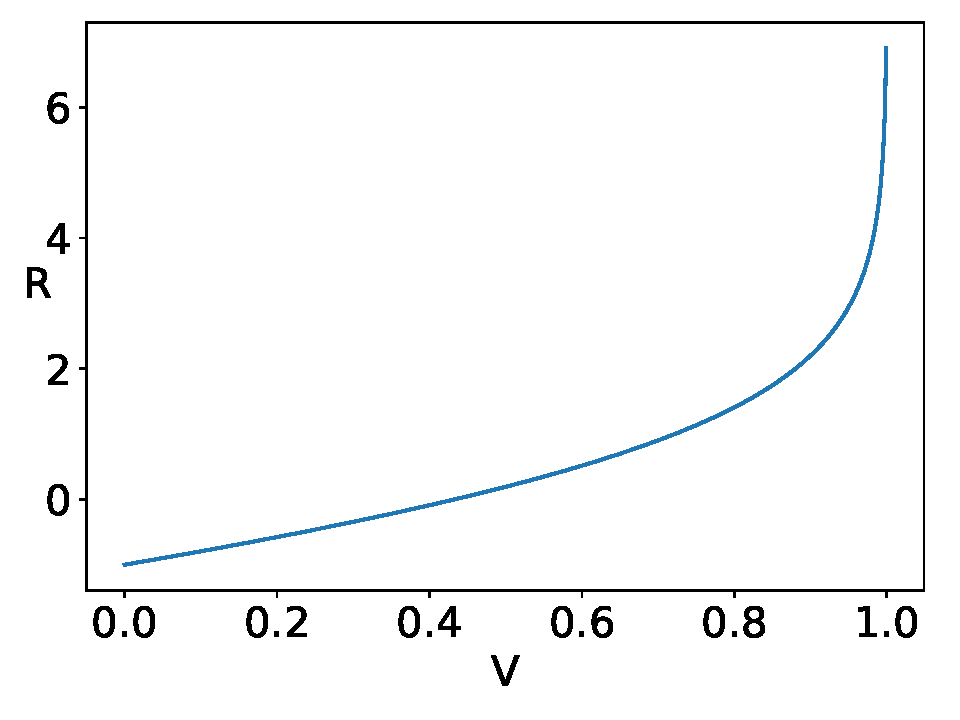
\includegraphics[scale=0.7]{images/reward_visib.pdf}
}
\caption{Зависимость функции награды от значения видности.}
\label{fig:reward_visib}
\end{figure}

\subsection{Архитектура нейронной сети агента}

Для параметризации $Q$-функции в работе использовалась нейронная сеть с архитектурой, предложенной в работе \cite{mnih2013atari}. Для работы с изображениями применяется 3-слойная сверточная нейронная сеть с параметрами (выходное число каналов, размер ядра, и сдвиг), равными [(32, 8, 4), (64, 4, 2), (64, 3, 1)] и функцией активации $ReLU$. Далее для обработки признаков, получаемых на выходе сверточной нейронной сети, использовался двухслойный перцептрон с функцией активации $ReLU$. Листинг задания нейронной сети DQN агента приведен в приложении \ref{lst:dqn}. 

\subsection{Параметры агента и обучение в симуляции}

При обучении DQN агента использовались стандартные параметры, совпадающие с параметрами, использованными в работе \cite{mnih2013atari}. Значения параметров приведены в таб.~\ref{tab:dqn_params}.

\begin{table} [htbp]
    \centering
    \begin{threeparttable}% выравнивание подписи по границам таблицы
        \caption{Параметры Double duelling DQN агента.}\label{tab:dqn_params}%
        \begin{tabular}{| p{5cm} || p{5cm} |}
            \hline
            \hline
            параметр & значение \\
            \hline
            total steps & $10^8$ \\
            $\varepsilon$-decay steps & $10^6$ \\
            rollout steps & 4 \\
            final $\varepsilon$ & 0.1 \\
            max grad norm & 50 \\
            batch size & 32 \\
            buffer size & $10^6$ \\
            init buffer size & $5 \cdot 10^4$ \\
            learning rate & $5 \cdot 10^{-4}$ \\
            gamma & 0.99 \\
            \hline
            \hline
        \end{tabular}
    \end{threeparttable}
\end{table}

                        
\section{Метод настройки с использованием непрерывного пространства действий}

Настройка интерферометра с использованием дискретного пространства действий имеет ряд ограничений. Размер шага агента фиксирован, что ограничивает качество настройки интерферометра. Также DQN агент вращает оптические элементы последовательно, что существенно уменьшает скорость настройки. Для настройки интерферометра с использованием непрерывных действий был выбран алгоритм TD3. Его можно рассматривать как обобщение алгоритма DQN на пространство непрерывных действий. Основной частью алгоритма TD3 является нейронная сеть, параметризующая стратегию агента $\pi_{\theta}(s_t)$, которая обучается предсказывать действия, максимизирующие значение $Q$-функции $\pi_{\theta}(s_t) = a_t: Q(s_t, a_t) \to \max$.

\subsection{Пространство действий}

Действия представляют собой вектор $a \in \mathcal{R}^5$. Компоненты вектора соответствуют угловым отклонениям обоих зеркал вокруг осей $x$ и $y$ и линейному смещению линзы относительно начального положения. Каждая компонента вектора действия лежит в интервале $[-1,1]$, где значения $\pm 1$ соответствуют максимальному и минимальному значениям из таб.~\ref{tab:MZI_params}, \ref{tab:MZI_lens_params}. В случае, если после применения действий суммарное смещение будет по модулю больше $1$, то его значение устанавливается равным соответственно $1$ или $-1$.
Амплитуда каждой компоненты вектора действия ограничиваются в интервале $[2.5 \cdot 10^{-3}, 1]$, так как действия меньшей амплитуды не приводят к видимому изменению интерференционной картины и лежат в пределах шумов пьезо моторов, используемых в механизированных подвижках.

\textbf{Масштабирование действий.} 
В процессе настройки агент должен оперировать все меньшими и более точными действиями. В среднем амплитуда действий в процессе настройки уменьшается на два порядка (как показано в разделе \ref{sec:ch2/sec8/subsec2}). Таким образом, шум, добавляемый в действия для исследования среды, также должен уменьшаться вместе с амплитудой действия. Для того чтобы удовлетворить этому условию, действия агента, полученные на выходе нейронной сети  $a\in[-1,1]$ преобразуем согласно уравнению:

\begin{equation}
a^{\prime} =
   \begin{cases}
    {\mathrm{sign}}(a) \cdot 1000^{|a| - 1}  & \quad \text{если $|a| > 0.17$} 
    \\
    0  & \quad \text{иначе}
  \end{cases}
\label{eq:rescale}
\end{equation}

\begin{figure}[ht]
\centerfloat{
    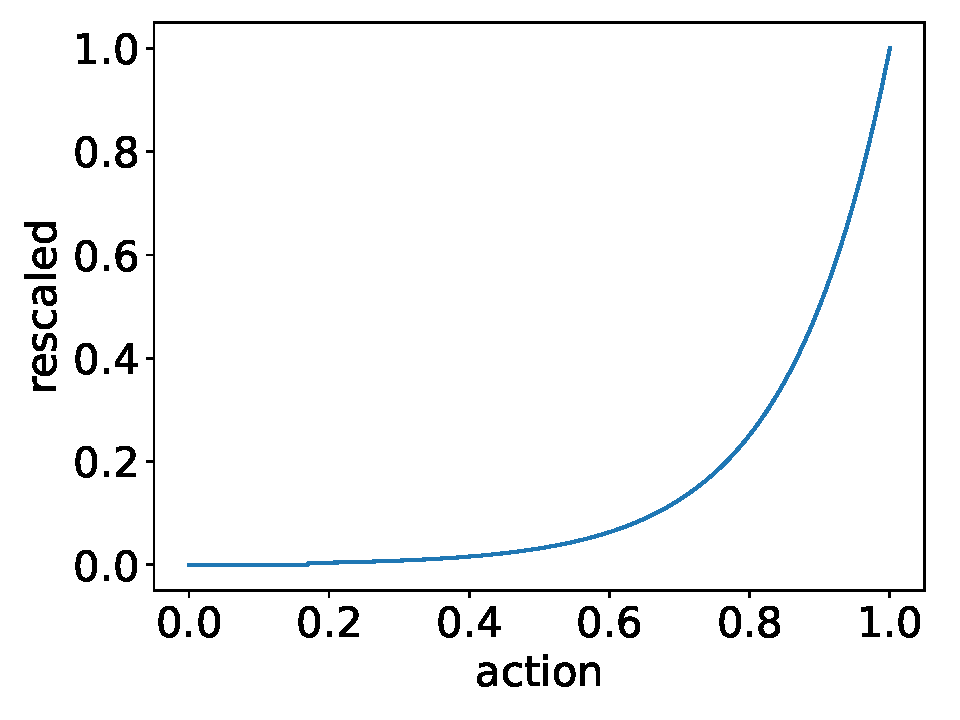
\includegraphics[scale=0.7]{images/rescale.pdf}
}
\caption{Преобразование пространства действий. Для действия $a > 0$.}
\label{fig:rescale}
\end{figure}

График преобразования \eqref{eq:rescale} представлен на рис.~\ref{fig:rescale}. Данное преобразование приводит к действиям с абсолютными значениями $|a|\in\{0\}\cup[2.5 \cdot 10^{-3}, 1]$. При обучении агента шум первоначально добавляется в ``сырые действия'' $a$, затем производится преобразование $a \to a^{\prime}$ согласно ур.~\eqref{eq:rescale}. При реализации масштабирования действий, действия $a$ хранятся в буфере в не преобразованном виде, а преобразуются в момент выполнения в среде. 

\subsection{Функция награды}

Аналогично алгоритму DQN, функция награды основана на преобразованном выражения для видности интерференционной картины:

\begin{equation}
    R = V - \log(1-V)  
\label{eq:td3_reward}
\end{equation}

В отличие от функции награды, использованной для обучения алгоритма DQN \eqref{eq:dqn_reward}, в функции награды $\eqref{eq:td3_reward}$ отсутствует слагаемое $-1$. Оно негативно влияло на процесс обучения TD3 агента. Если агент во время обучения производит действия, которые переводят один из управляющих элементов в крайнее положение в соответствии с указанным в таблицах \ref{tab:MZI_params}, \ref{tab:MZI_lens_params}, эпизод считается завершенным для предотвращения повреждения оптических элементов. В дополнение к завершению эпизода агент получает отрицательную награду $r_p=-0.04$. Данная награда важна в начале обучения агента, когда основная награда  \eqref{eq:td3_reward} обычно близка к нулю. Небольшая отрицательная награда за не безопасные действия задает агенту понимание границ среды, но не останавливает процесс исследования среды. Величина награды $r_p$ была подобрано вручную в процессе экспериментов. С другой стороны, когда агент достаточно обучился настройке интерферометра, он обычно получает значительную положительную награду на каждом шаге настройки. В этом случае раннее завершение эпизода будет иметь значительное негативное влияние на суммарную дисконтированную награду, и, таким образом, вероятность небезопасных действий сильно уменьшается.

\subsection{Архитектура нейронной сети агента}

При обучении TD3 агента использовались параметры, приведенные в разделе \ref{sec:ch2/sec4/subsec4}. В качестве кодировщика для преобразования изображений интерференционной картины латентное пространство в обоих нейронных сетях актора и критика мы использовали архитектуру VGG-16 \cite{simonyan2014very} с 8 сверточными слоями. Латентный вектор, получаемый после кодировщика, затем обрабатывается трехслойным перцептроном. Данная архитектура была выбрана из-за операций пуллинга (max pooling), которые помогают уменьшить переобучение и чувствительность к шумам в отдельных пикселях входных изображений. Листинг задания нейронной сети актора приведен в приложении \ref{lst:td3}. При обучении мы использовали ортогональную инициализацию весов всех моделей, так как она способствовала более быстрой сходимости.

\subsection{Параметры агента и обучения в симуляции}\label{sec:ch2/sec4/subsec4}

Мы обучали агента с коэффициентом дисконтирования награды $\gamma = 0.8$. Такое значение $\gamma$ соответствует горизонту $\Delta$ (числу шагов, при котором из-за дисконтирования будущая награда будет близка к $0$) равному: 

\begin{equation}
    \Delta = \frac{1}{1 - \gamma} = 5
\end{equation}

Горизонт $\Delta$ = 5 примерно равен числу шагов, требуемому агенту для достижения существенного значения видности $\gamma > 0.6$. 

Мы добавляли нормально распределенный шум в действия до масштабирования со стандартным отклонением, уменьшающимся экспоненциально с $0.5$ до $0.02$ в течение процесса обучения агента. Несмотря на то, что дисперсия шума не зависит от амплитуды действия $a$, его эффект на действие, выполняемое в среде $a^{\prime}$, зависит от амплитуды из-за преобразования \eqref{eq:rescale}. Суммарное число шагов в среде при обучении агента равно $10^6$, а размер буфера равен $10^5$. Обновления весов выполнялись каждые десять шагов агента. Процесс обучения с использованием видеокарты NVidia RTX 2080 занял 26 часов. 

\begin{table} [htbp]
    \centering
    \begin{threeparttable}% выравнивание подписи по границам таблицы
        \caption{Параметры TD3 агента.}\label{tab:td3_params}%
        \begin{tabular}{| p{5cm} || p{5cm} |}
            \hline
            \hline
            параметр & значение \\
            \hline
            total steps & $10^6$ \\
            noize std start & $0.5$ \\
            noize std final & $0.02$ \\
            max grad norm & $10$ \\
            batch size & 32 \\
            buffer size & $10^5$ \\
            init buffer size & $10^4$ \\
            $\pi$ learning rate & $10^{-5}$ \\
            $q$ learning rate & $10^{-4}$ \\
            $\gamma$ & 0.8 \\
            $\rho_{\mathrm{polyak}}$ & 0.995 \\
            num\_epochs & 10  \\
            policy\_delay & 1 \\
            $\sigma_{\mathrm{targ}}$ & 0.2 \\
            $c$ & 0.5 \\
            \hline
            \hline
        \end{tabular}
    \end{threeparttable}
\end{table}

        

\section{Программно-аппаратный комплекс Интерферобот}

Перед тем как перейти к анализу результатов работы агентов на экспериментальной установке, опишем общую структуру разработанного программно-аппаратного комплекса, его основные характеристики и отличительные особенности. Программно-аппаратный комплекс получил название Интерферобот. Программная часть комплекса состоит из симулятора работы оптического интерферометра, пользовательского интерфейса, обученного агента машинного обучения с подкреплением. Аппаратная часть состоит из механизированных подвижек, применяемых для управления оптическими элементами интерферометра. 

\begin{figure}[ht]
\centerfloat{
    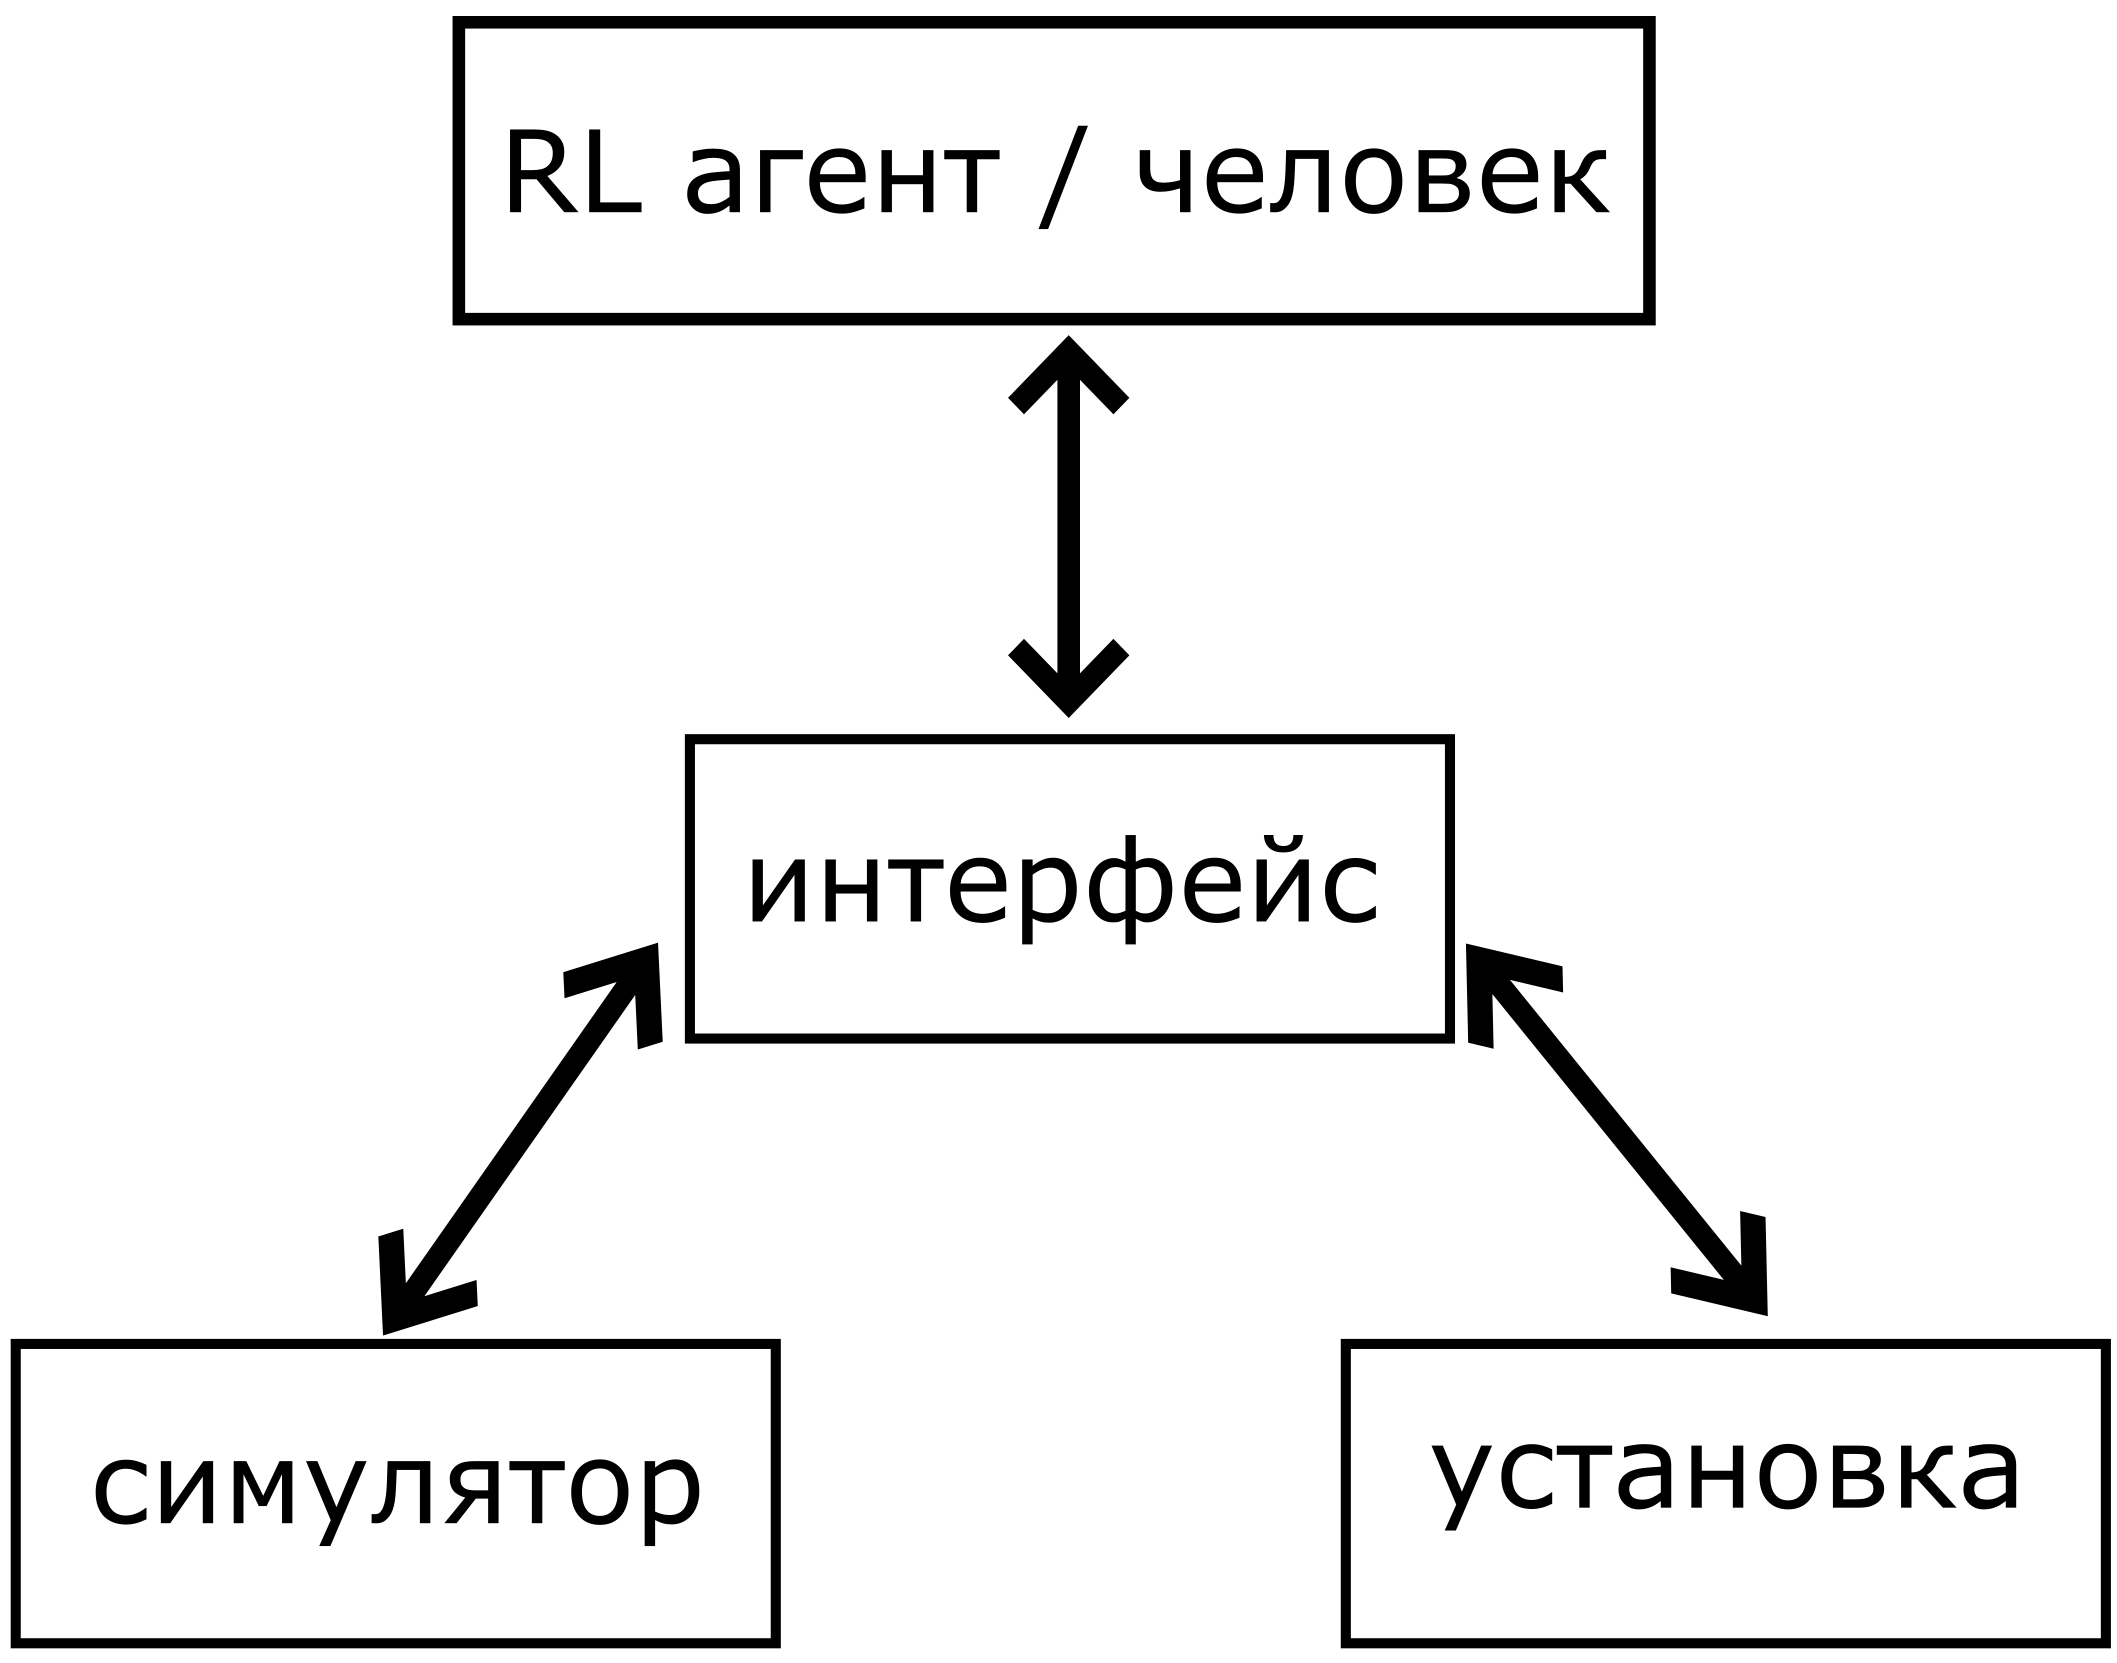
\includegraphics[scale=0.5]{images/interferobot_complex.png}
}
\caption{Схема взаимодействия модулей в программно-аппаратном комплексе Интерферобот.}
\label{fig:interf_complex}
\end{figure}

Схема взаимодействия модулей в комплексе Интерферобот представлена на рис.~\ref{fig:interf_complex}. В нем RL агент или человек используют один и тот же интерфейс как для взаимодействия с симулятором интерферометра, так и с физической установкой. Отличительно чертой разработанного программно-аппаратного комплекса является то, что он не специализирован под конкретный тип интерферометра и может быть легко использован для настройки различных типов интерферометров. Для адаптации к другому типу интерферометра нужно изменить модель интерферометра в симуляторе и обучить соответствующего RL агента. Благодаря тому, что интерфейс симулятора и экспериментальной установки стандартизирован, агент обученный на симуляторе может быть без изменений запущен на физической установке. 

\paragraph{Симулятор оптического интерферометра Маха-Цендера.}
Математическая и численная модели, лежащие в основе симулятора, описаны в разделе \ref{sec:ch2/sec1}. Для обучения RL агентов симулятор имеет стандартный gym интерфейс \cite{brockman2016openai}. Симулятор реализован на языках программирования Python3 и С++. Трекинг лучей через систему линз и зеркал и интерфейс для взаимодействия с RL агентом реализована на языке программирования Python3. Для ускорения работы симулятора вычисление интерференционной картины как наиболее вычислительно сложная часть, реализована на C++ с использованием параллельных вычислений. Взаимодействие между C++ и Python3 осуществляется с помощью библиотеки ctypes. Благодаря такой архитектуре и использованию параллельных вычислений симулятор с использованием 16 потоков на персональном компьютере с процессором intel core i7 рассчитывает 200 состояний среды (16 изображений 64х64 пикселя) за одну секунду. 

\paragraph{Пользовательский интерфейс.}

Для настройки интерферометра с помощью человека и отладки работы симулятора был разработан графический интерфейс пользователя, приведенный на рис.~\ref{fig:gui}. 

\begin{figure}[ht]
\centerfloat{
    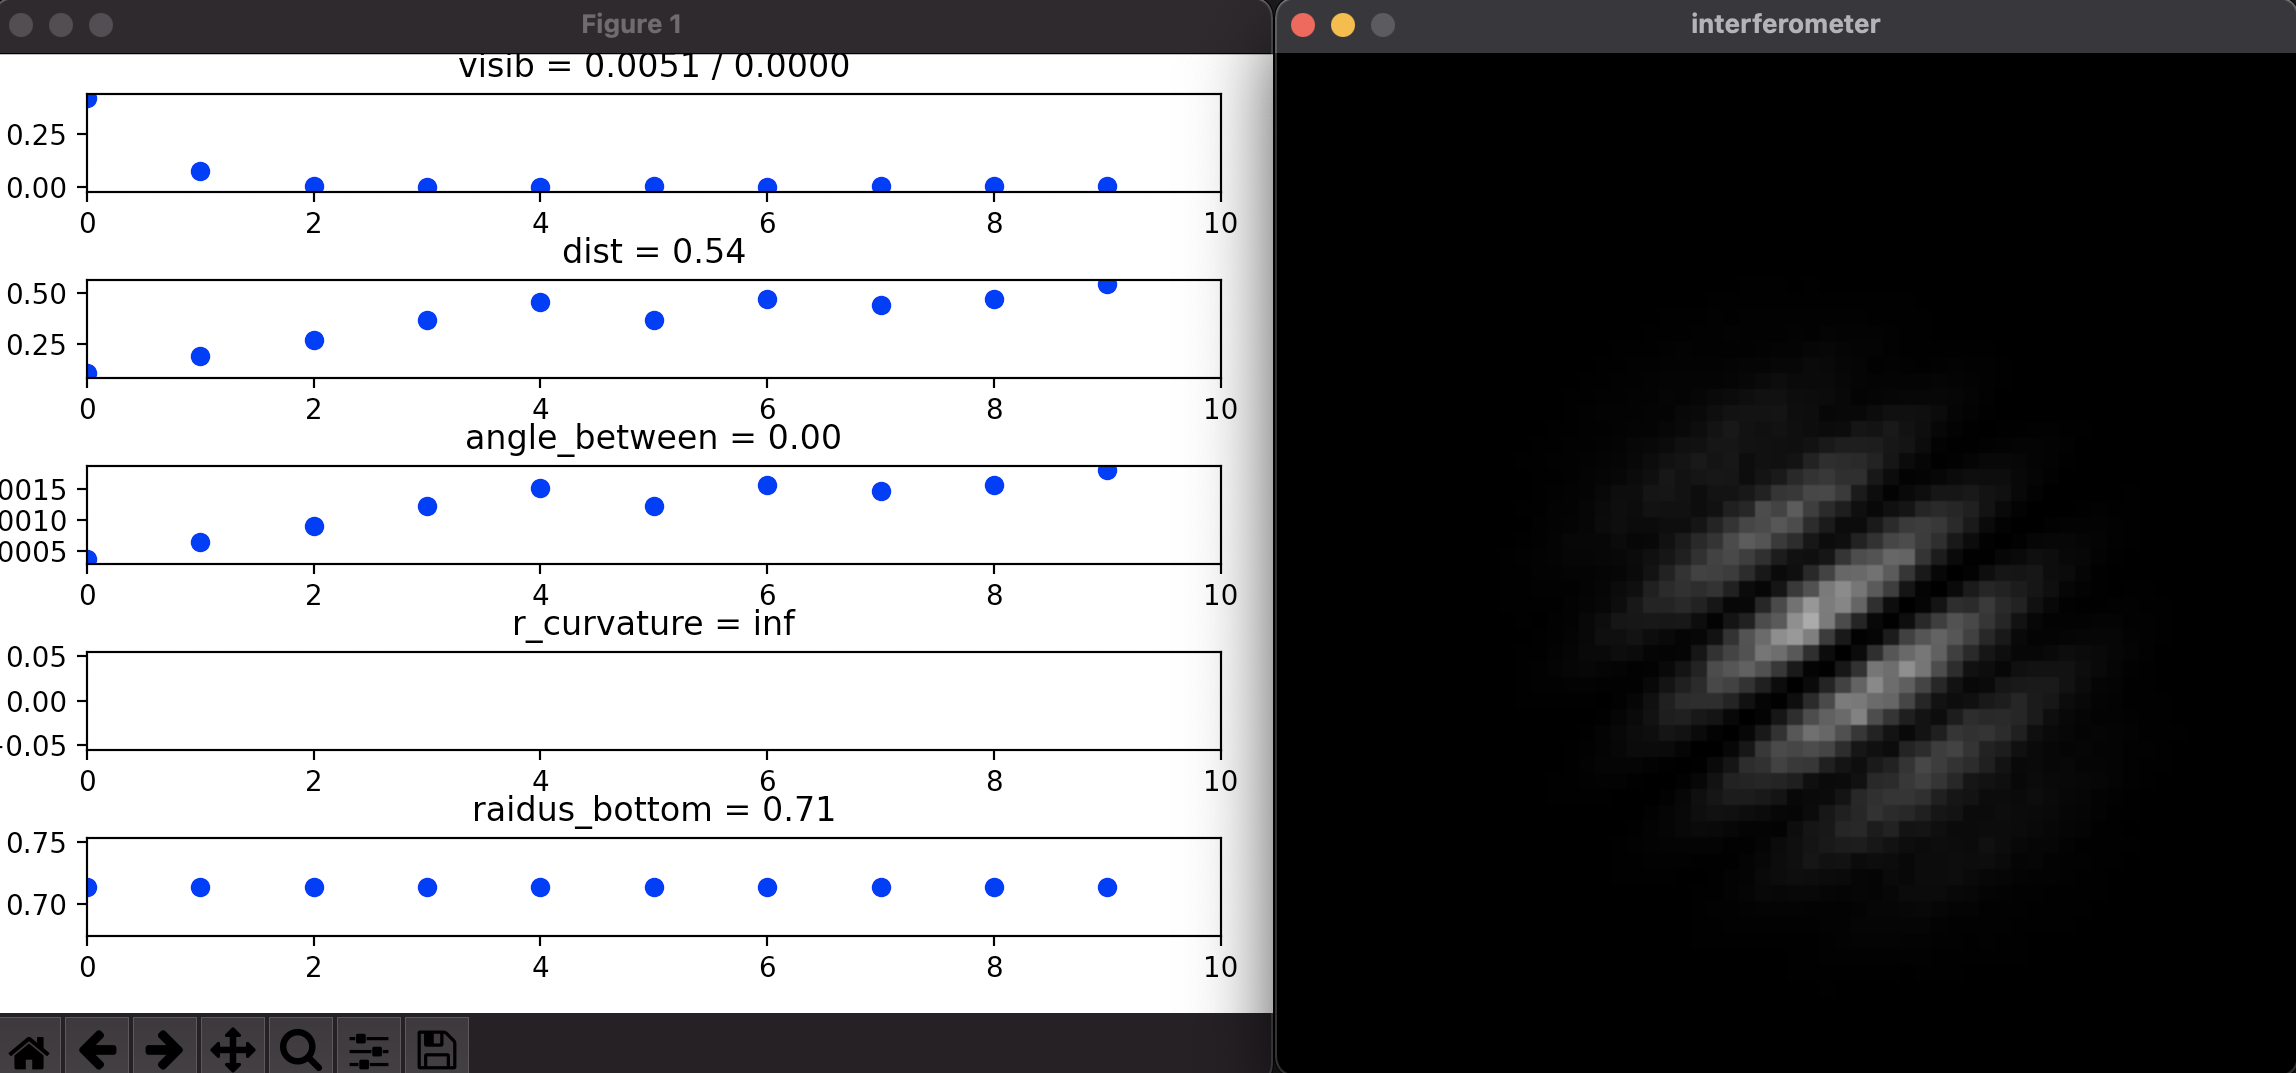
\includegraphics[scale=0.45]{images/gui.png}
}
\caption{Графический интерфейс пользователя.}
\label{fig:gui}
\end{figure}

Пользовательский интерфейс программы состоит из двух окон. В левом окне показаны значения метрик, таких как видность интерференционной картины, расстояние и угол между пучками, радиус кривизны волнового фронта и радиус пучка в динамике в процессе настройки интерферометра. В правом окне показана интерференционная картина. Управление производится с помощью клавиатуры. Клавиши $i,j,k,l$ управляют поворотами светоделителя $BS\ 2$ в двух плоскостях на положительный и отрицательный угол. Клавиши $w,a,s,d$ аналогично управляют поворотами зеркала $mirror\ 1$. Для управления положением линзы служат клавиши $m,n$. Включение и выключение RL агента производится по нажатию на клавишу пробел. По нажатию на клавишу $r$ происходит расстройка интерферометра и начало нового эпизода. Клавиши $1,2,3$ используются для изменения амплитуды действий.

\paragraph{Экспериментальная установка.} Экспериментальная установка интерферометра Маха-Цендера без линз, соответствующая схеме \ref{fig:MZI}, представлена на рис.~\ref{fig:MZI_exp}. 

\begin{figure}[ht]
\centerfloat{
    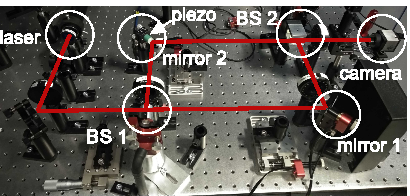
\includegraphics[scale=2.3]{images/interf_real_1.pdf}
}
\caption{Экспериментальная установка интерферометра Маха-Цендера соответствующая схеме \ref{fig:MZI}.}
\label{fig:MZI_exp}
\end{figure}

Геометрические параметры установки, максимальные углы отклонения зеркал и радиус пучков приведены в таб.~\ref{tab:MZI_params}. Для определения радиуса, распределение интенсивности пучка, полученное в эксперименте, было аппроксимировано в соответствии с ур.~\eqref{eq:I_def}. Мы использовали гелий-неоновый  лазер с длинной волны $\lambda =  635$ нм, управляемые подвижки для зеркал Newport, камеру IDS UI-2230SE-M-GL с пространственным разрешением $1600\times1200$ пикселей, временным разрешением 18 кадров в секунду и матрицей размером $3.57\times4.76$ мм. Полученные изображения затем были обрезаны до размера $1200\times1200$ и масштабированы к разрешению $64\times64$ пикселя с использованием библиотеки opencv.

\paragraph{Измерение параметров пучка.}
Для симуляции работы экспериментальной установки необходимо задать параметры пучка. Для измерения радиуса мы сняли изображение одного пучка и аппроксимировали его следующим распределением: $y = \left( A \cdot \exp(-(x - x_0)^2 / r^2) \right) ^2$. Квадрат Гауссовой функции был использован для моделирования распределения яркости на изображении пучка, так как яркость изображения пропорциональна интенсивности света, которая, в свою очередь, является квадратом амплитуды напряженности электромагнитного поля. Изображения экспериментального и аппроксимированного пучков представлены на рис~\ref{fig:rad_fit}(a,b). 

\paragraph{Ошибка измерения видности.}
Мы определили величину инструментальной ошибки вычисления видности по изображениям интерференционной картины. Мы сравнили видность, рассчитанную этим методом, с видностью, рассчитанной с использованием фотодиода. Фотодиод может быть представлен как камера только с одним пикселем, но с очень большим временным разрешением, благодаря чему можно получить интегральное значение интенсивности света с большей дискретизацией и точнее оценить его размах. Стандартное отклонение видности, вычисленной с использованием камеры и с использованием фотодиода, составило $0.02$.

При использовании линз согласно схеме \ref{fig:MZI_expl_lenses} геометрические параметры интерферометра сохраняются. Был уменьшен первоначальный размер пучков на выходе из лазера. Линзы были выбраны с одинаковым фокусным расстоянием, равным 50 мм. Расстояние от светоделителя $BS\ 1$ до первой линзы также равно 50 мм. Параметры приведены в таб.~\ref{tab:MZI_lens_params}. 


Автоматизированное управление интерферометром осуществляется с помощью персонального компьютера под управлением ОС Ubuntu. Управление подвижками зеркал производилось с помощью библиотеки libusb \cite{libusb}. Для управления подвижкой линзы использовалась библиотека xilab \cite{standa_soft}. Для получения изображений с камеры использовалась библиотека ueye \cite{ids_soft}. 

\section{Перенос из симуляции в реальность}\label{sec:ch2/sec6}

Изображения интерференционной картины и динамика среды у симулятора и физической установки существенно отличаются. В эксперименте на изображениях присутствуют аберрации, паразитная интерференция, засветка сторонними источниками света, а также профиль светового пучка отличается от Гауссова. Механизированные подвижки движутся не точно и имеют значительный гистерезис. Поэтому для того, чтобы успешно перенести агента из симуляции на физическую установку, мы добавили в симуляцию шумы, основанные на неопределенности в измерениях.

\begin{figure}
\centering
  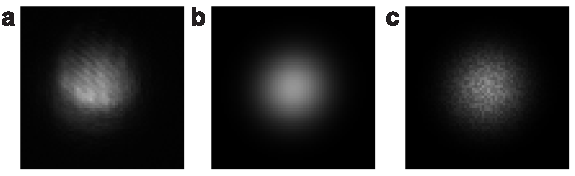
\includegraphics[width=0.8\linewidth]{images/beamsamples.pdf}

\caption{Одиночные лазерные лучи: (a) экспериментальный, (b) модель, (c) модель с шумом. На рис.(a) полосы видны из-за эффекта резонатора на защитном стекле камеры.}
\label{fig:rad_fit}
\end{figure}


\paragraph{Шумы применяемые в начале каждого эпизода.} 
\begin{itemize}
    \item \textbf{radius randomization}. При проведении эксперимента точное измерение радиуса пучка не всегда возможно. Также форма пучка часто может отличаться от Гауссова профиля, используемого в модели. Для того чтобы учесть это отличие между симулятором и экспериментом, мы в процессе обучения агента случайным образом изменяем радиус пучка на $\pm 20\%$. Случайный выбор радиуса пучка также помогает учесть отличие экспериментального профиля пучка от модельного. Экспериментальный пучок показан на рис.~\ref{fig:rad_fit}(a), модельный пучок показан на рис.~\ref{fig:rad_fit}(b).
\end{itemize}

\paragraph{Шумы применяемые на каждом шаге взаимодействия со средой.}
\begin{itemize}
    \item \textbf{exposure randomization}. Яркость интерференционного изображения зависит от времени выдержки камеры, используемой при проведении эксперимента. Мы случайным образом изменяем яркость интерференционной картины на $\pm 30\%$ для того, чтобы агент мог адаптироваться к различному времени выдержки камеры.
    \item  \textbf{image noise}. Из рис.~\ref{fig:rad_fit}(a) видно, что в изображении экспериментального пучка содержится шум, могут быть пылинки и наблюдаться паразитная интерференция. Для того чтобы дать агенту информацию о шумах в изображениях, мы добавляем $20\%$ белого шума в каждый пиксель итогово изображения (рис.~\ref{fig:rad_fit}(с)). 
    \item \textbf{cycle frame shift}. Наблюдением являются 16 последовательных изображений, полученных за один проход пьезо зеркала. При этом стартовая точка у пьезо зеркала может быть любой. Для того чтобы учесть произвольное стартовое положение пьезо зеркала, мы применяем циклический сдвиг на случайную величину к последовательности из 16 интерференционных изображений. 
    \item \textbf{duty cycle randomization}. Для того чтобы агент мог адаптироваться к соотношению времени прямого и обратного проходов пьезо зеркала мы случайным образом изменяем их длительность. При этом процент изображений, полученных в течении прямого прохода, поддерживается больше половины (не меньше 9 из 16) для того, чтобы агент получал достаточно информации для определения направления движения интерференционных полос.  
    \item \textbf{phase noise}. Также важным фактором является то, что разность фаз между последовательными интерференционными изображениями не является постоянной. График, демонстрирующий зависимость интенсивности интерференционной картины в зависимости от номера кадра, показан на рис.~\ref{fig:piezo_noise}. Видно, что экспериментальная зависимость отличается от модельной зависимости наличием глубоких провалов. Это происходит в следствии неравномерного движения пьезо зеркала и флуктуаций плотности воздуха, которые приводят к случайным изменениям в длине оптического пути лучей в двух плечах интерферометра. Для учета данного эффекта мы добавили нормально распределенный шум со стандартным отклонением, равным $0.5$ рад. к разности фаз двух лучей. Таким образом, фаза для каждого из $k$ кадров выбирается случайным образом из распределений $\mathcal{N}(\frac{2\pi k}{N_{\mathrm{forw}}}, 0.5)$, $\mathcal{N}(\frac{2\pi k}{N_{\mathrm{backw}}}, 0.5)$ в зависимости от направления прохода, где $N_{\mathrm{forw/backw}}$ --- число изображений, снимаемых за время прямого и обратного проходов соответственно.
\end{itemize}

Фазовый шум был добавлен только для обучения DQN и TD3 агентов на интерферометре Маха-Цендера с системой линз.

Мы не добавляем шум в действия агента при обучении для моделирования проскальзывания подвижек, используемых для управления оптическими элементами. При условии, что шум в проскальзывании является независимыми и несмещенным, то он не будет влиять на величину оптимального действия. 
Однако при тестировании шум в действиях может быть использован для оценки надежности работы агента.


\begin{figure}
  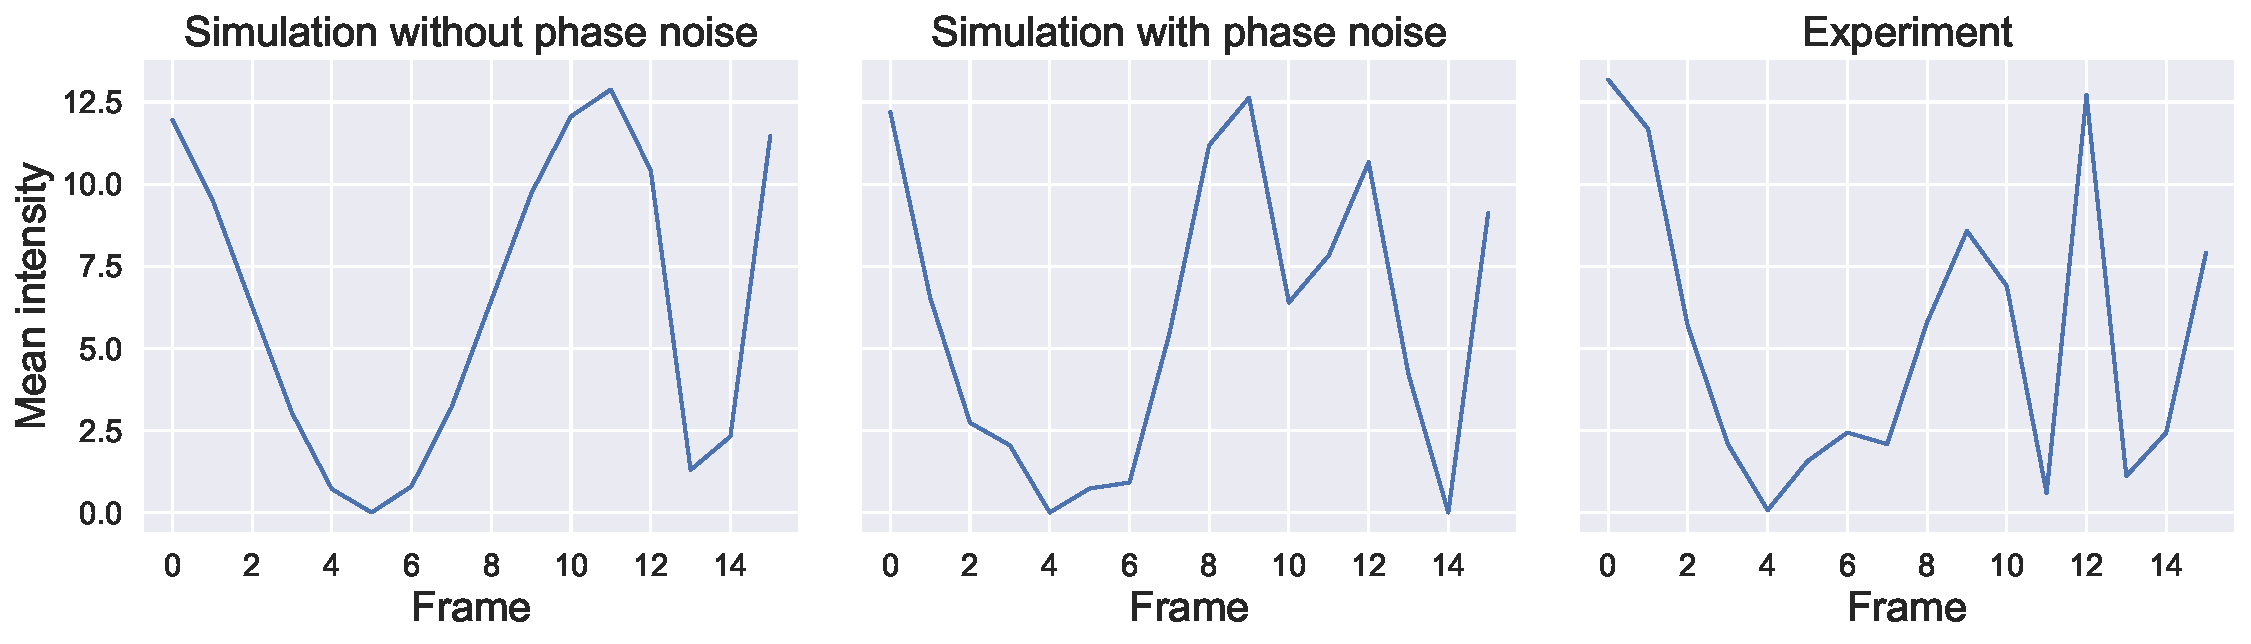
\includegraphics[width=1\linewidth]{images/Piezo_noise.pdf}
  \centering
  \caption{Эффект фазового шума. Суммарная интенсивность интерференционной картины в зависимости от номера кадра. Добавление фазового шума делает симуляцию ближе к зависимости наблюдаемой в эксперименте.}
  \label{fig:piezo_noise}
\end{figure}


\section{Настройка интерферометра Маха-Цендера без линз}

\subsection{Оценка результатов работы агента на экспериментальной установке}
Для экспериментальной оценки качества работы агента использовалась установка, показанная на рис.~\ref{fig:MZI_exp}. Мы реализовали для нее gym интерфейс \cite{brockman2016openai}, который позволяет запускать без изменения RL агента, обученного в симуляции. В качестве наблюдений для RL агента мы использовали 16 последовательных изображений интерференционной картины, получаемых с камеры за один период прохода пьезо зеркала. Видность интерференционной картины вычислялась средой напрямую из интерференционных изображений. Время, требуемое для получения одного состояния на экспериментальной установке, составило $2.7$ секунды. Таким образом, экспериментальная установка медленнее симулятора более чем в $400$ раз. Агент был протестирован в автоматическом режиме без участия человека в течении $100$ эпизодов по $100$ шагов каждый. В начале каждого эпизода интерферометр был расстроен в случайное начальное положение. 

\begin{figure}[ht]
\centerfloat{
    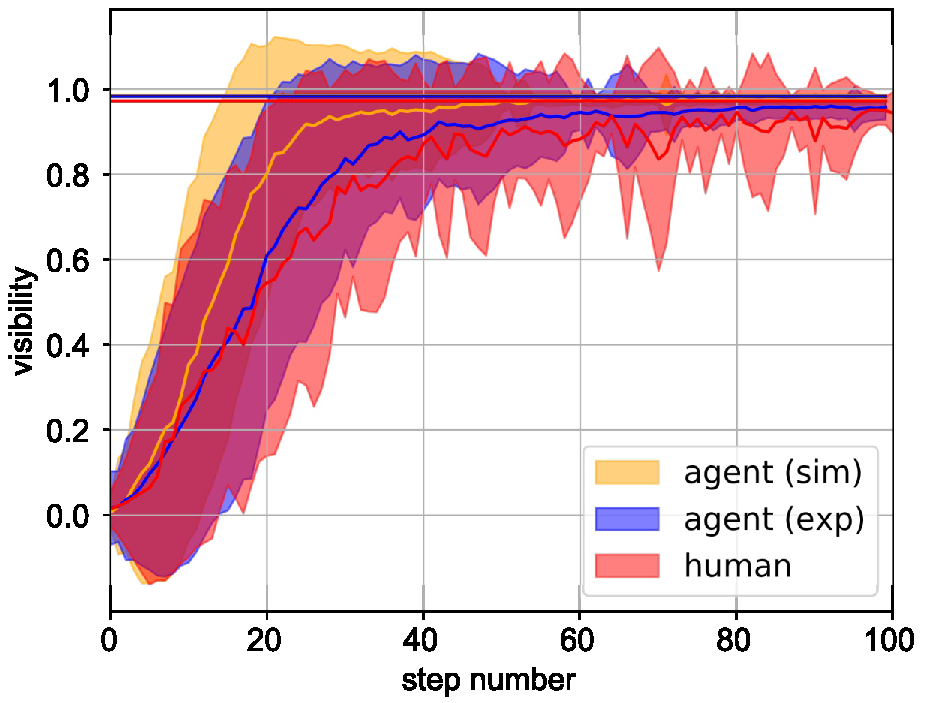
\includegraphics[width=0.8\textwidth]{images/eval1_visib_step.pdf}
}
\caption{Сравнение настройки интерферометра DQN агентом в симуляции и на экспериментальной установке с человеком, использующим клавиатуру. Результаты работы агента усреднены по 100 эпизодам, человека --- по 18.}
\label{fig:eval_visib_step}
\end{figure}

На рис.~\ref{fig:eval_visib_step}, \ref{fig:eval_visib_time} мы представили результаты работы DQN агента усредненные по 100 тестовым эпизодам настройки интерферометра и сравниваем качество работы агента с настройкой интерферометра опытным экспериментатором. Человек производил настройку интерферометра в двух постановках:  

\begin{itemize}
    \item с использованием клавиатуры, совершая действия такой же величины, как и RL агент. 
    \item вращая зеркала с помощью ручек, также как и при проведении оптических экспериментов.
\end{itemize}

Рис.~\ref{fig:eval_visib_step} соответствует первой постановке. В дополнение к DQN агенту, настраивающему экспериментальную установку (изображен красным цветом), мы также показываем результаты агента в симуляции (синим цветом) для сравнения. Видно, что качество работы агента в симуляции слегка выше, чем в эксперименте, из-за отличий между симулированной средой и физической установкой. Несмотря на это, DQN агент превосходит человека, использующего тот же набор действий, как показано на рис.~\ref{fig:eval_visib_step}. В качестве дополнительной метрики рассмотрим наибольшее значение видности, достигнутое в каждом эпизоде и затем усредненное по всем эпизодам, представленное в таб.~\ref{tab:highest_visib_dqn}. Также следует заметить, что человек настраивает интерферометр с помощью клавиатуры сильно медленнее по времени, чем DQN агент. 

\begin{table} [htbp]
    \centering
    \begin{threeparttable}
        \caption{Средняя наибольшая видность достигнутая при настройке интерферометра.}\label{tab:highest_visib_dqn}
        \begin{tabular}{| p{5cm} || p{5cm} || p{5cm} |}
            \hline
            \hline
            DQN (sim) & DQN (exp) & Human \\
            \hline
            0.986 & 0.983 & 0.972 \\
            \hline
            \hline
        \end{tabular}
    \end{threeparttable}
\end{table}

Похожие результаты были получены и во второй постановке [рис.~\ref{fig:eval_visib_time}]. Так как в данном случае сложно разделить процесс настройки интерферометра человеком на дискретные шаги, строим видность в зависимости от времени, потраченного на настройку. В этом случае среднее максимальное значение видности, достигнутой человеком, равно $0.968$. Из рис.~\ref{fig:eval_visib_time} видно, что человек в среднем превосходит DQN агента в начале каждого эпизода, но отстает в процессе тонкой настройки. Также видно, что стандартное отклонение у эксперта в начале настройки установки меньше, чем у DQN агента, но к середине настройки оно становится сильно больше. 

\begin{figure}[ht]
\centerfloat{
  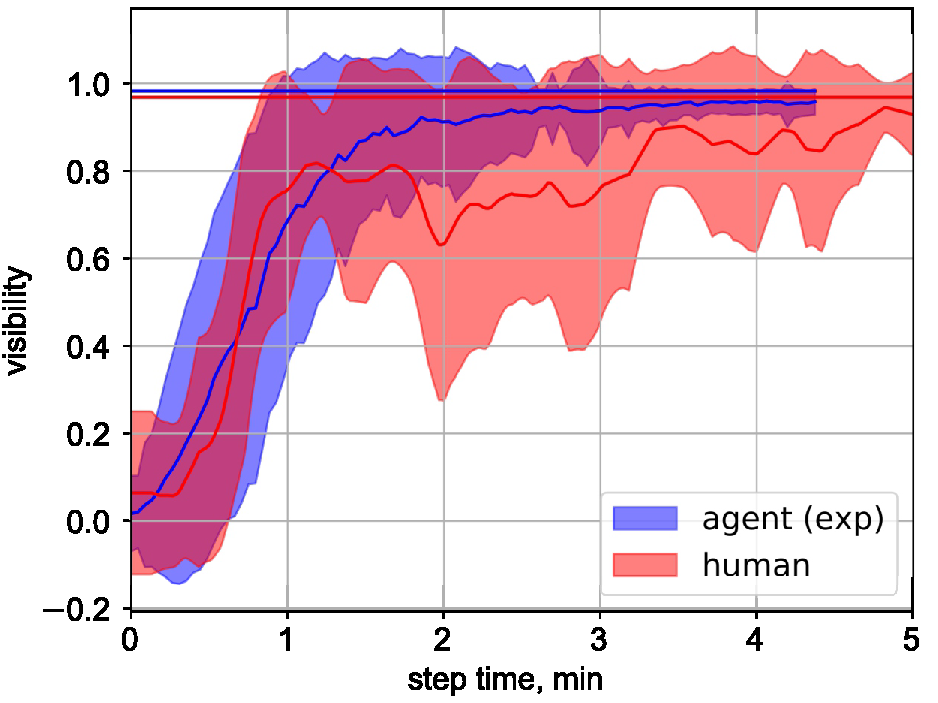
\includegraphics[width=0.8\textwidth]{images/eval1_visib_time.pdf}
}
\caption{Сравнение настройки интерферометра DQN агентом в симуляции и на экспериментальной установке с человеком, непосредственно вращающим зеркала. Результаты работы агента усреднены по 100 эпизодам, человека --- по 16.}
\label{fig:eval_visib_time}
\end{figure}

Эксперт настраивает оптический интерферометр, анализируя изображения интерференционной картины (см. приложение \ref{app:C}). В начале настройки, когда интерферометр сильно расстроен, эксперту просто интерпретировать полосы на интерференционных изображениях и выполнить быструю настройку за несколько действий. Однако, после этого эксперт не способен надежно различать небольшую разницу в положении центров пучков $(x_0,y_0)$ на камере. Для того чтобы увидеть эту разницу, он отодвигает пучок далеко в сторону, что приводит к временному уменьшению видности интерференционной картины. Такое падение видности не наблюдается в первой постановке на рис.~\ref{fig:eval_visib_step}. В первой постановке при использовании клавиатуры для того, чтобы сильно раздвинуть пучки в интерферометре,  требуется совершить большое количество дискретных действий. Поэтому человек использует другую стратегию: поворот двух зеркал на равный угол, что приводит к перемещению центра настраиваемого пучка без изменения угла между пучками. Данный подход часто применяется экспериментаторами на практике при настройке оптических устройств и имеет название ``beam walk''. 


\subsection{Анализ стратегии используемой агентом при настройке интерферометра}

\begin{figure}[ht]
\centerfloat{
  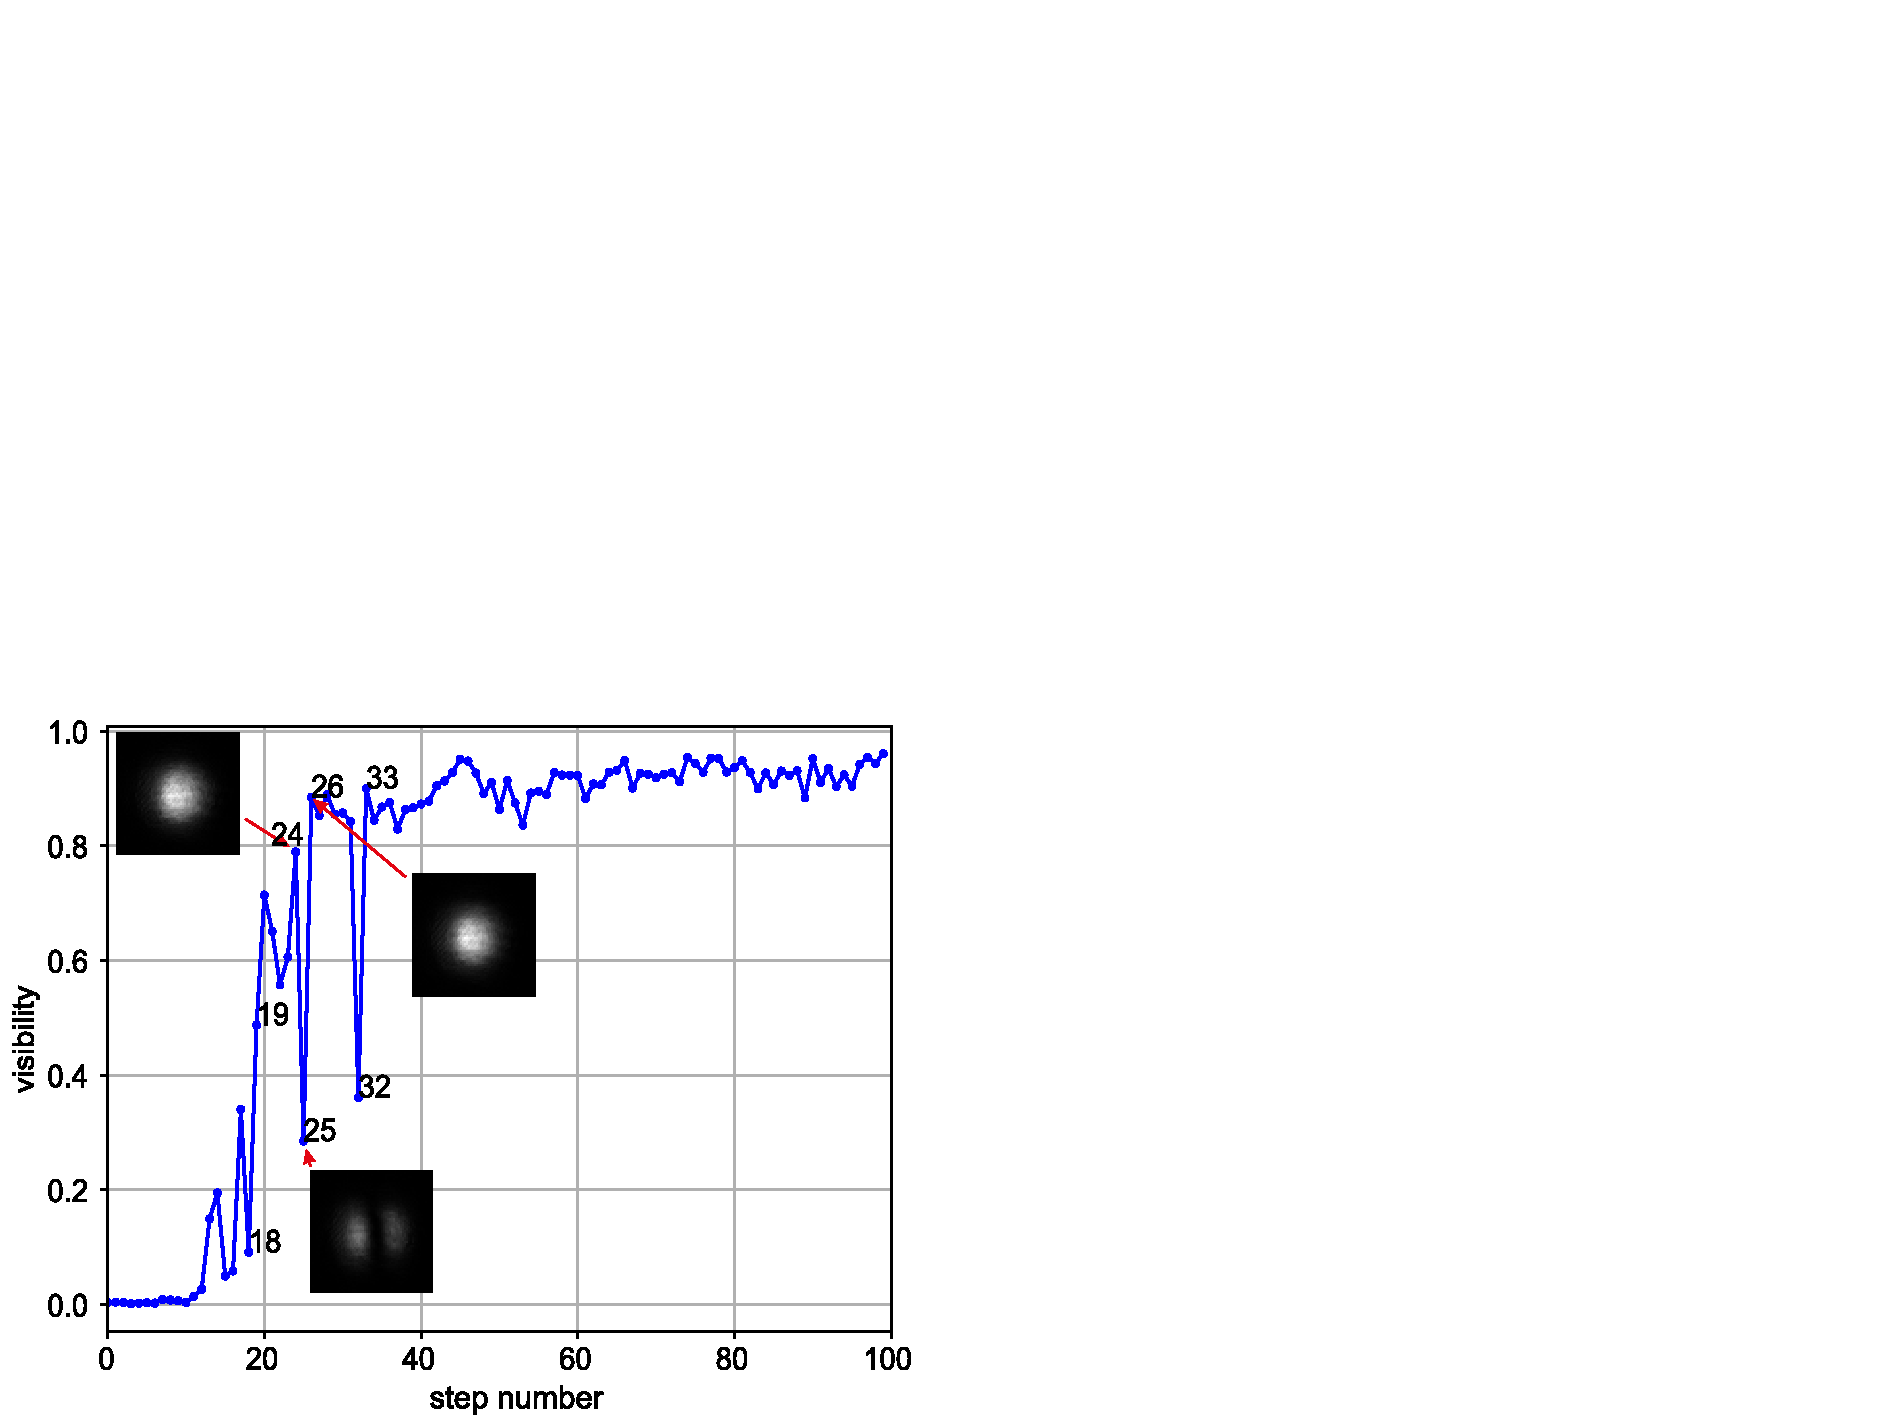
\includegraphics[width=0.8\textwidth]{images/anal1_visib_step.pdf}
}
\caption{Изменение видности в одном эпизоде настройки интерферометра. Интерференционные изображения на снимках соответствуют 24, 25 и 26 шагам настройки интерферометра. 
}
\label{fig:anal_visib_step}
\end{figure}

\begin{figure}[ht]
\centerfloat{
  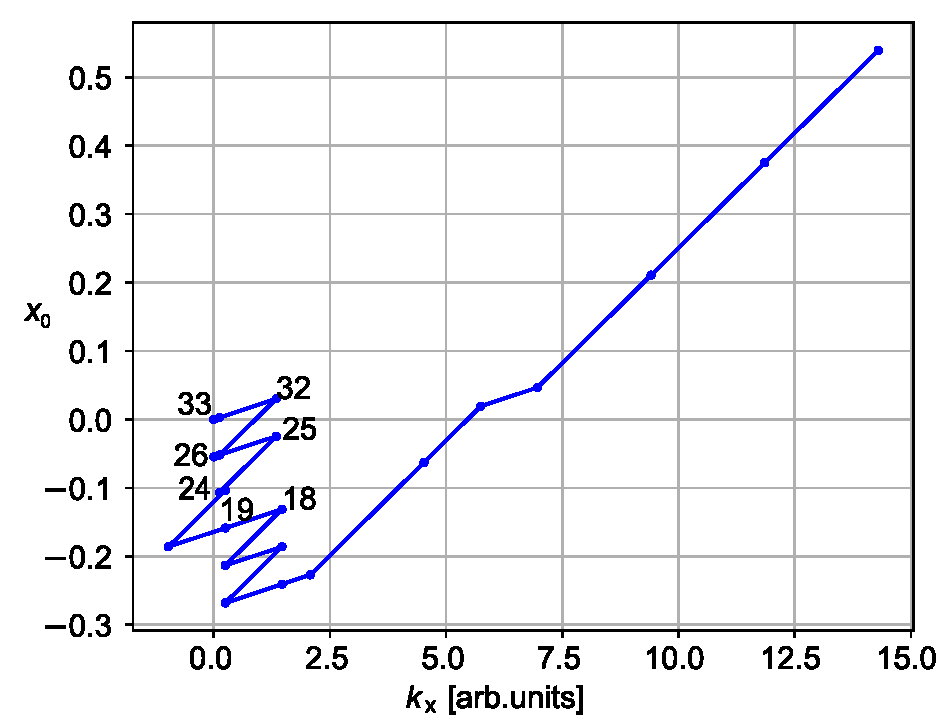
\includegraphics[width=0.8\textwidth]{images/anal1_kx.pdf}
}
\caption{Траектория в фазовом пространстве, соответствующая эпизоду настройки интерферометра, показанному на рис.~\ref{fig:anal_visib_step}. Траектория в пространстве $(x, k_x)$ последовательно сходится к настроенному состоянию.}
\label{fig:anal_kx}
\end{figure}

RL агент старается достичь состояния с максимальной видностью  $(x_0,y_0,k_x,k_y)$ согласно ур.~\eqref{eq:visib_rot}, за наименьшее количество шагов. Так как действия агента изменяют одновременно положение центра $(x_0, y_0)$ и направление пучка $(k_x k_y)$, то они не являются ортогональными в этом пространстве (уменьшение пространственного расстояния между пучками может увеличить угловое и наоборот). Таким образом, оптимальная стратегия не может увеличивать видность на каждом шаге настройки интерферометра. Оптимальный RL агент должен производить тонкую настройку интерферометра, последовательно отклоняя одно зеркало и компенсируя это вторым зеркалом. Такое поведение будет приводить к существенному изменению видности в течении настройки, как видно на рис.~\ref{fig:anal_visib_step}, \ref{fig:anal_kx}. Важным отличием стратегии агента, показанной на рис.~\ref{fig:anal_visib_step}, от эксперта, является то, что человек расстраивает интерферометр для того, чтобы лучше определить положение пучков, а RL агент совершает последовательные повороты двух зеркал для того, чтобы подстроить положение центра пучка $x_0$ или $y_0$ без изменения его направления ($k_x$, $k_y$). Таким образом, вместо того, чтобы действовать жадно, агент расстраивает интерферометр, для того чтобы настроить его лучше на следующем шаге. Это поведение не было запрограммировано, а было выучено агентом полностью самостоятельно в симуляции.  Рис.~\ref{fig:anal_kx} показывает траекторию настройки интерферометра в фазовом пространстве, соответствующую видности изображенной на рис.~\ref{fig:anal_visib_step}. Так как мы не знаем точных значений  $x_0, y_0$, и $k_x, k_y$ в эксперименте, мы их реконструируем, исходя из того, что в конце настройки $(x_0, y_0) = (0, 0)$ и $(k_x, k_y) = (0, 0)$. На рис.~\ref{fig:anal_kx} видно, что в начале агент настраивает установку большими шагами, а затем зигзагообразно сдвигает пучки вместе.

На рис.~\ref{fig:step_size} показан средний размер шага DQN агента (в единицах $\alpha_{\max}$) в течении эпизода как функция номера шага. Видно, что в начале настройки агент совершает действия с большой амплитудой, затем в конце для точной настройки агент делает наименьшие действия. 

\begin{figure}[ht]
\centerfloat{
  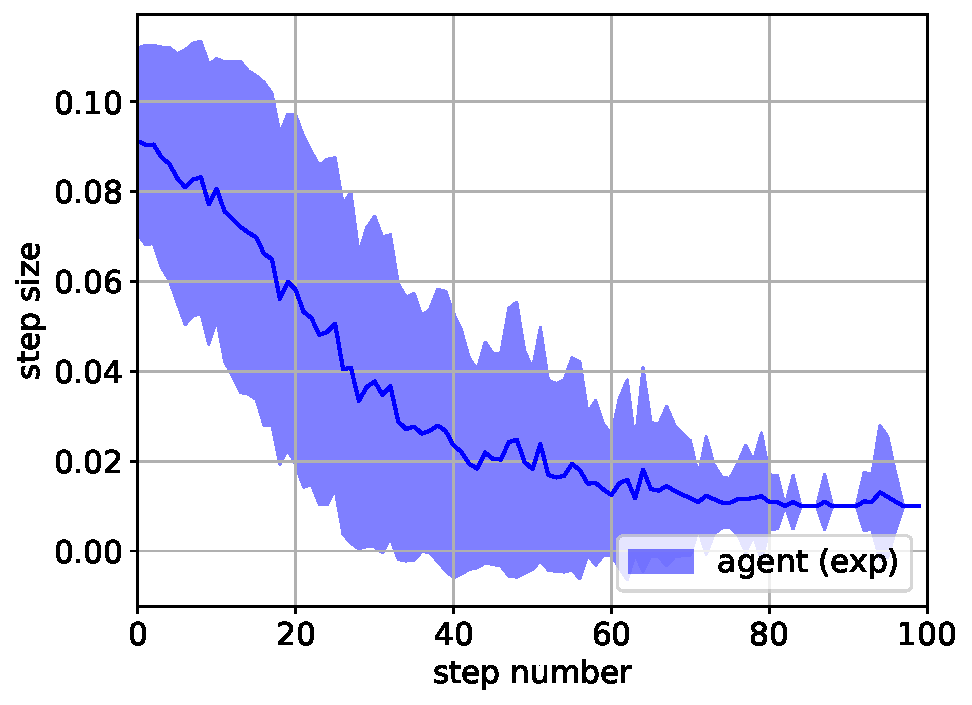
\includegraphics[width=0.75\textwidth]{images/agent_step_size.pdf}
}
\caption{Размер шага DQN агента усредненный по 100 эпизодам.}
\label{fig:step_size}
\end{figure}

\subsection{Анализ эффективности шумов использованных при обучении}

Для того чтобы определить важность использования шумов при обучении DQN агента, мы обучили и протестировали четырех агентов, при обучении каждого из которых один из шумов, перечисленных в разделе \ref{sec:ch2/sec6}, был убран. Каждый агент был протестирован в $100$ эпизодах. Процесс тестирования каждого агента занимал порядка 6 часов и был полностью автоматизирован. В таблице \ref{tab:abl}, мы представили среднюю видность, полученную агентом в течении последних 20 шагов настройки интерферометра (visibility) и среднюю суммарную дисконтированную награду, полученную агентом (return). Наибольший прирост производительности агента при настройке физической установки обеспечивают шумы в радиусе и белый шум. 

\begin{table} [htbp]
    \centering
    \begin{threeparttable}
        \caption{Анализ влияния шумов используемых при обучении агента на качество настройки физической установки.}\label{tab:abl}
        \begin{tabular}{| p{10cm} || p{3cm} || p{3cm} |}
            \hline
            \hline
             & visibility & return \\
            \hline
            All randomizations  & $\textbf{0.96} \pm \textbf{0.02}$ & $\textbf{221} \pm \textbf{54}$ \\
            No radius randomization & $0.74 \pm 0.20$ & $85 \pm 69$ \\
            No exposure randomization& $0.91 \pm 0.04$ & $178 \pm 39$ \\
            No image noise & $0.82 \pm 0.07$ & $129 \pm 43$ \\
            No duty cycle and frame shift randomization  &  $0.89 \pm 0.07$ & $200 \pm 42$ \\
            \hline
            \hline
        \end{tabular}
    \end{threeparttable}
\end{table}


\section{Настройка интерферометра Маха-Цендера с системой линз}

\subsection{Оценка результатов работы агента на экспериментальной установке}

Для тестирования работы TD3 и DQN агентов при настройке интерферометра Маха-Цендера с системой линз была построена экспериментальная установка, соответствующая схеме, изображенной на рис.~\ref{fig:MZI_expl_lenses}. Для определения видности интерференционной картины использовался фотодетектор с большим временным разрешением. Каждого агента мы тестировали на $50$ эпизодах длинной в $100$ шагов. Результаты тестирования представлены на рис.~\ref{fig:results_a}, \ref{fig:results_b}. TD3 агент, использующий непрерывное пространство действий, настраивает интерферометр существенно лучше, чем DQN агент, оперирующий дискретными действиями. На рис.~\ref{fig:results_a} показана зависимость видности интерференционной картины от шага настройки интерферометра. Видно, что TD3 агент не только значительно быстрее достигает хорошей видности (так как он оперирует действиями произвольного размера), но и имеет меньший разброс и лучшее качество в конце настройки. На рис.~\ref{fig:results_b} показан межквантильный размах для видности, усредненной по последним 40 шагам в каждом эпизоде. Видно, что также у TD3 агента размах значений видности существенно меньше, чем у DQN агента.

\begin{figure}[ht]
\centerfloat{
    \includegraphics[width=0.75\textwidth]{images/DQN_vs_TD3.pdf}
}
    \caption{Видность в зависимости от шага настройки интерферометра усредненная по 50 эпизодам.  TD3 агент показан синим цветом, DQN --- оранжевым.}
    \label{fig:results_a}
\end{figure}

\begin{figure}[ht]
\centerfloat{
        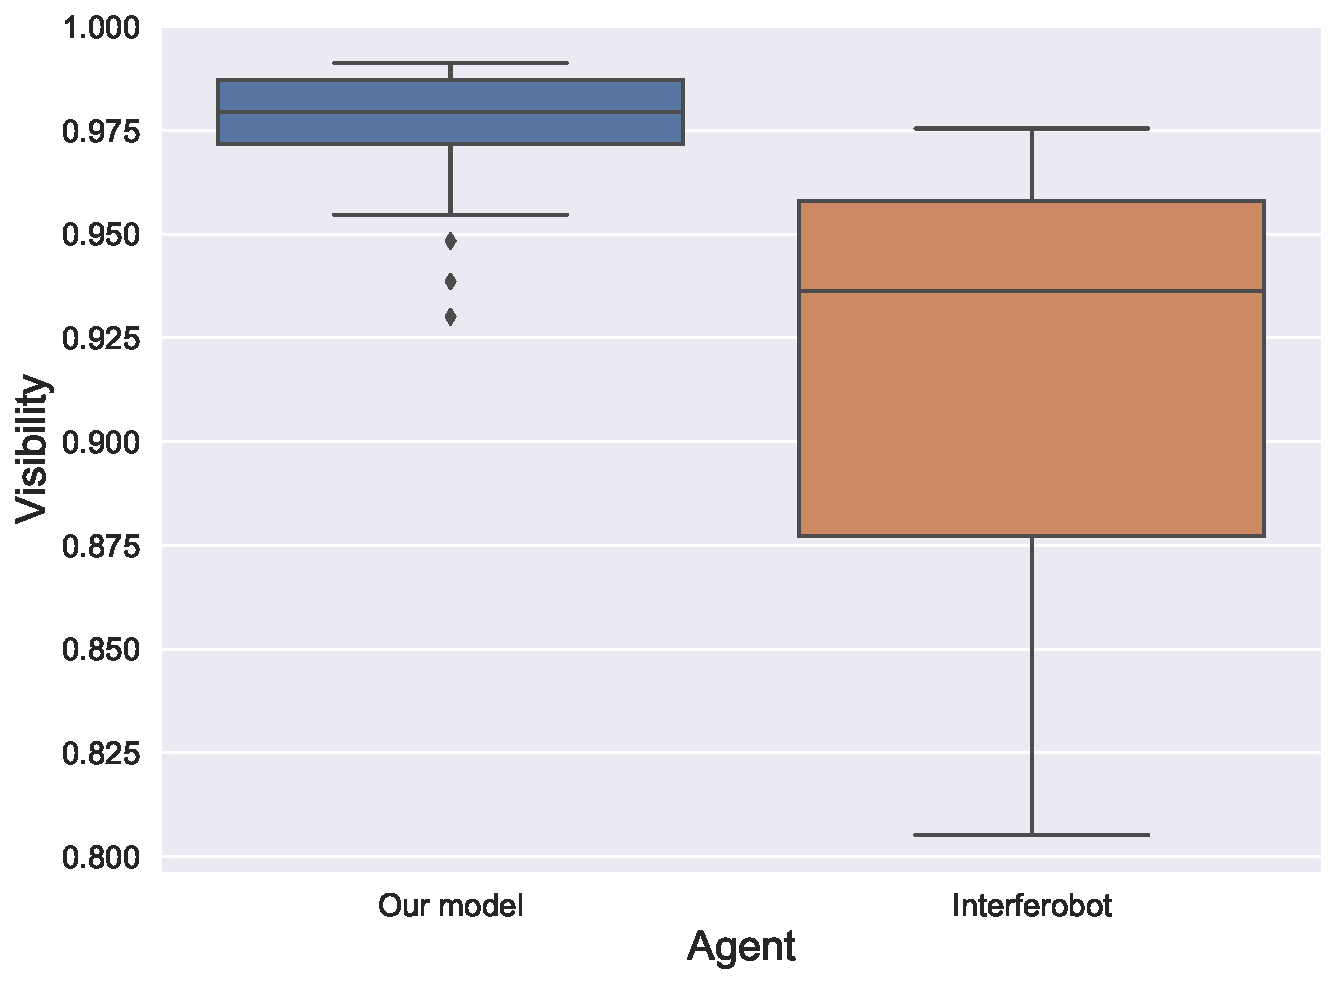
\includegraphics[width=0.75\textwidth]{images/DQN_vs_TD3_box.pdf}
}
\caption{Межквантильный размах видности, полученной в конце настройки интерферометра. Межквантильный размах определяется как разность между 25 и 75 перцентилями.}
    \label{fig:results_b}
\end{figure}

В таб.~\ref{tab:human} представлено сравнение качества настройки интерферометра с линзами RL агентами с экспертом. Эксперт настраивал интерферометр вручную $10$ раз, используя управляющие элементы подвижек зеркал и линзы. Видно, что TD3 агент также превосходит эксперта как в скорости, так и в качестве настройки.

\begin{table} [htbp]
    \centering
    \begin{threeparttable}
        \caption{Сравнение качества настройки интерферометра экспертом, TD3 и DQN агентами. Показано время в секундах, требуемое для достижения величины видности, равной $0.92$, $0.95$ и $0.98$. В скобках указан процент эпизодов, при в которых соответствующая видность не была достигнута.}\label{tab:human}
        \begin{tabular}{| p{4cm} || p{4cm} || p{4cm} || p{4cm} |}
            \hline
            \hline
            &V $\ge 0.92$ & V $\ge 0.95$ & V $\ge 0.98$ \\
            \hline
            Human &  93.9 (\textbf{0\%})  & 103.6 (\textbf{0\%}) & 129.6 (10\%)\\
            TD3 &  \textbf{56.16} (\textbf{0\%}) & \textbf{75.06} (\textbf{0\%}) & \textbf{120.1} (\textbf{4\%})\\
            DQN &  98.7 (7.6\%) & 116.1 (7.6\%) & 156.4 (10.6\%)\\
            \hline
            \hline
        \end{tabular}
    \end{threeparttable}
\end{table}

\subsection{Анализ стратегии используемой агентом при настройке интерферометра}\label{sec:ch2/sec8/subsec2}

Для настройки интерферометра необходимо точно совместить два пучка как по положению на камере, так и по направлению. Сложность этого процесс состоит в том, что каждое из двух зеркал изменяет как положение центра пучка, так и его направление. Для того чтобы перемещать пучок по экрану, сохраняя угол между двумя пучками, необходимо поворачивать два зеркала на один и тот же угол. На рис.~\ref{fig:anal2_parallel_actions} показано, что TD3 агент выучивает подобные действия и часто их использует: к концу процесса настройки интерферометра около 70\% процентов всех действий составляют ``параллельные действия''. 

\begin{figure}[ht]
\centerfloat{
  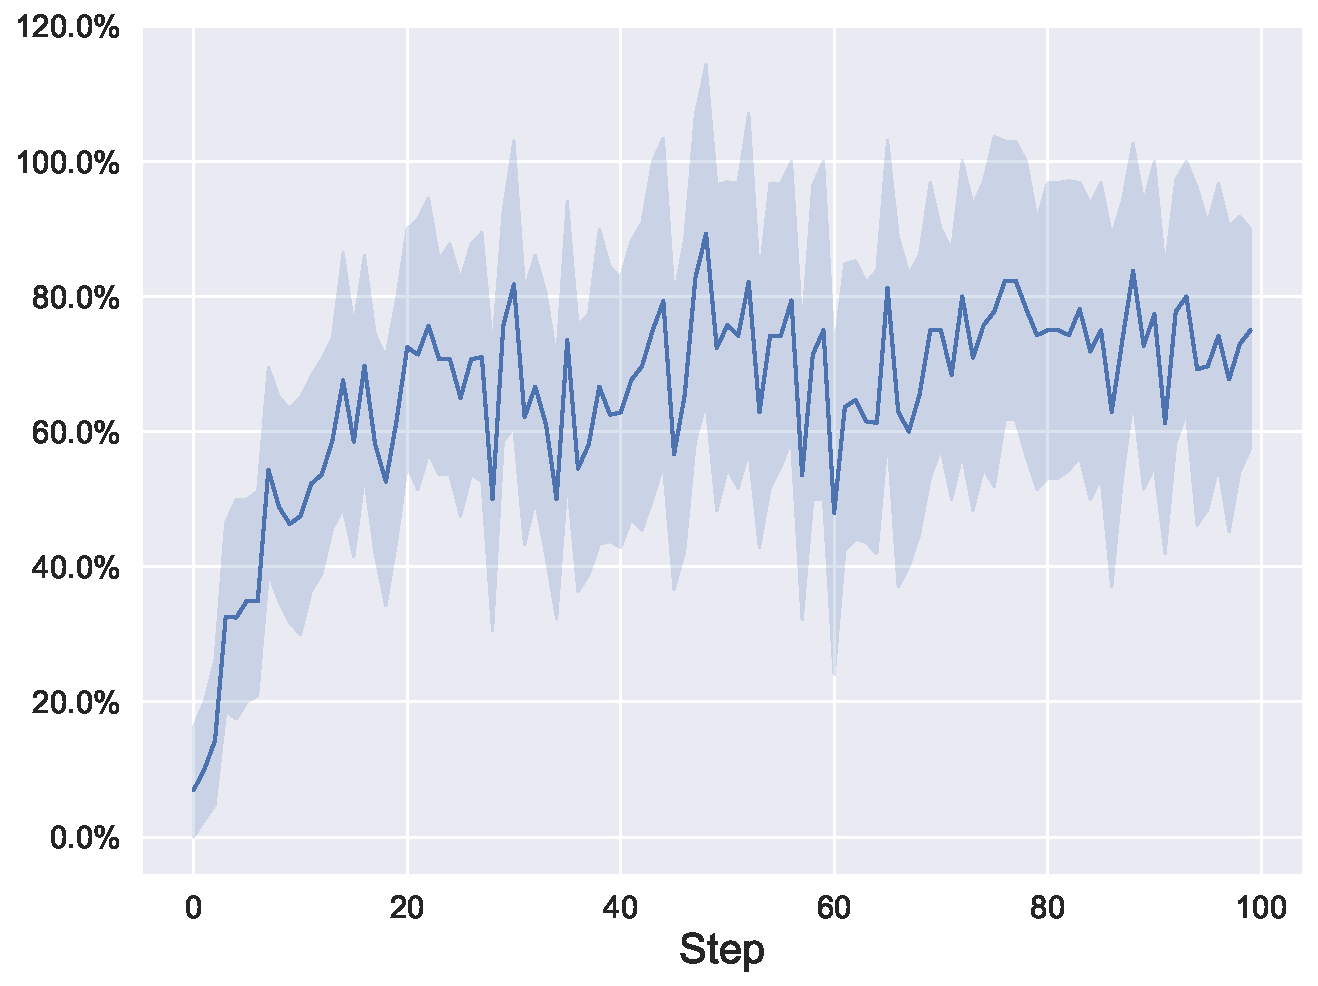
\includegraphics[width=0.75\textwidth]{images/parallel_actions_count_for_each_axis.pdf}
}
\caption{Процент ``параллельных действий'' --- действий, которые изменяют расстояние между лучами, не изменяя при этом угол между лучами в зависимости от номера шага.}
\label{fig:anal2_parallel_actions}
\end{figure}

Рис.~\ref{fig:anal2_act_norm} показывает усредненную зависимость амплитуды действий агента от номера шага настройки интерферометра. Амплитуда действий у TD3 (как и у DQN агента, рис.~\ref{fig:step_size}) убывает, так как в начале агент использует действия большой амплитуды для грубой настройки интерферометра, а затем с помощью малых действий производит тонкую настройку. 

\begin{figure}[ht]
\centerfloat{
  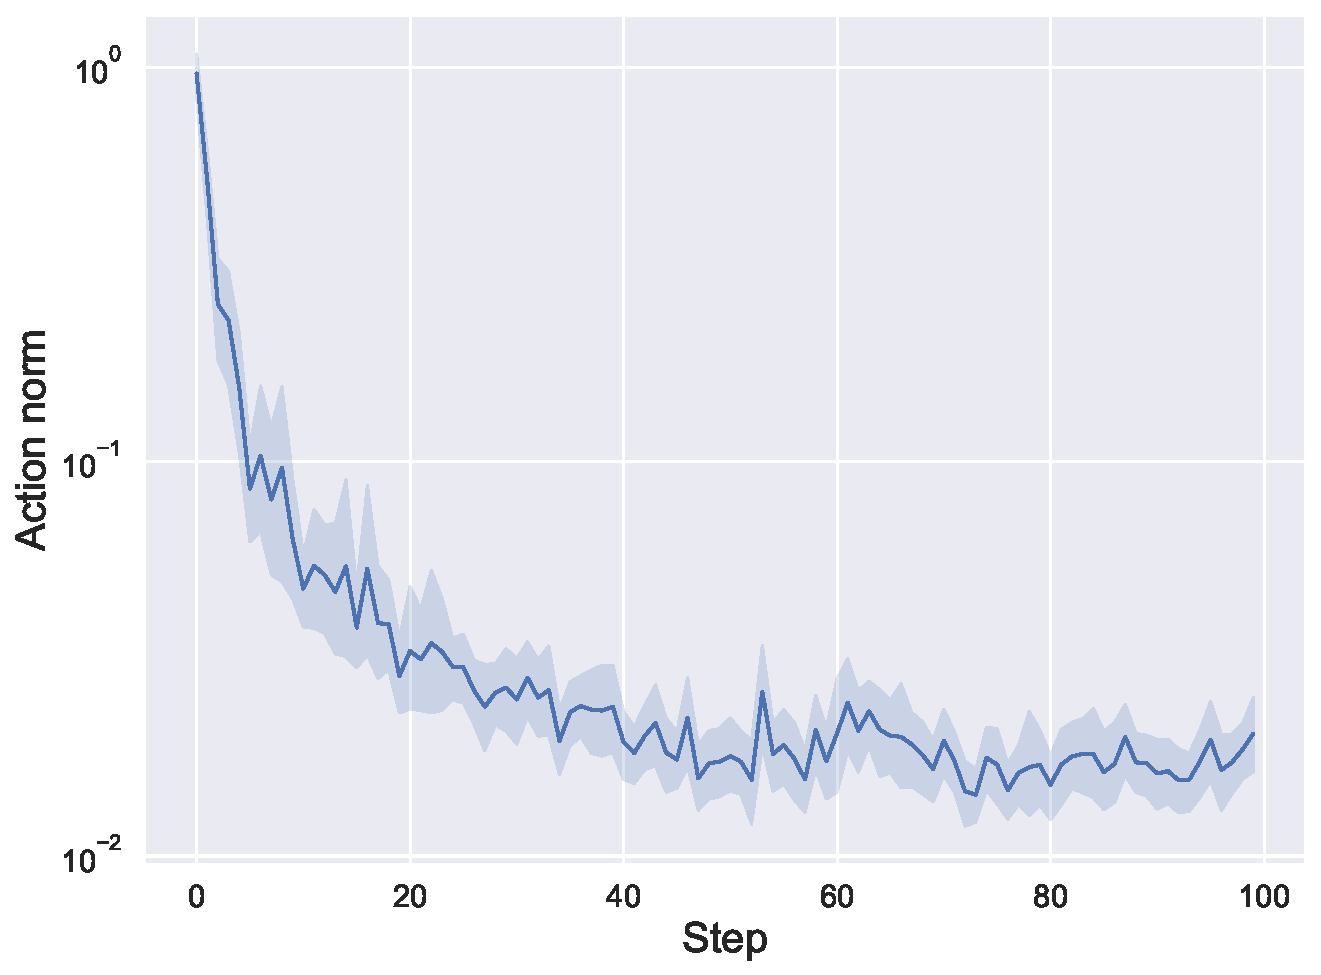
\includegraphics[width=0.75\textwidth]{images/action_norm_decrease.pdf}
}
\caption{Средняя амплитуда действий в зависимости от номера шага.}
\label{fig:anal2_act_norm}
\end{figure}


\subsection{Анализ эффективности шумов использованных при обучении}

В таблице \ref{tab:abl_td3} представлены результаты сравнения работы TD3 агента, обученного без использования фазового шума или масштабирования действий. Стандартный TD3 агент при настройке интерферометра показал качество хуже, чем DQN агент, и достиг видности равной $V = 0.83$. Масштабирование пространства действий и добавление фазового шума при обучении TD3 агента существенно улучшают качество его работы, приводя к видности $V = 0.98$. Также важно отметить, что фазовый шум слегка уменьшает среднюю видность, достигаемую DQN агентом, но также уменьшает дисперсию. Такой компромисс между дисперсией и смещением (bias-variance tradeoff) может быть связан с достаточной простотой нейронной сети, используемой в DQN агенте. 

\begin{table} [htbp]
    \centering
    \begin{threeparttable}
        \caption{Анализ эффективности фазового шума и масштабирования действий. PN --- фазовый шум, AR --- масштабирование действий.}\label{tab:abl_td3}
        \begin{tabular}{| p{4cm} || p{6cm} || p{6cm} |}
            \hline
            \hline
            агент & средняя видность за последние 40 шагов & стандартное отклонение \\
            \hline
            TD3 + AR + PN & \textbf{0.98} & \textbf{0.03} \\
            TD3 + AR & 0.95 & 0.06\\
            DQN + PN & 0.90 & 0.08\\
            TD3& 0.83 & 0.18\\
            \hline
            \hline
        \end{tabular}
    \end{threeparttable}
\end{table}

\section{Выводы}

Мы показали, что оптический интерферометр Маха-Цендера может быть успешно настроен RL агентом, обученным без каких либо априорных знаний о физике системы. 
Мы разработали программно-аппаратный комплекс Интерферобот, который позволяет обучать RL агента полностью в симуляции и затем применять для настройки физического интерферометра. В рамках работы мы предложили набор шумов, которые позволяют перенести обученного агента из симуляции на физическую установку без дополнительного дообучения. Для обучения агента в симуляции мы предложили функцию награды, которая позволяет агенту различать состояния с близкой видностью и достигать хорошего качества настройки интерферометра. 
Мы рассмотрели и реализовали два подхода к дискретизации пространства действий: дискретный (DQN агент) и непрерывный (TD3 агент). Качество настройки интерферометра с использованием дискретных действий находится на одном уровне с экспертом. Качество работы обученного агента с использованием непрерывного пространства действий превосходит качество настройки оптического интерферометра опытным экспертом как по скорости настройки, так и по получаемой в конце настройки видности интерференционной картины. 
Разработанный программно-аппаратный комплекс может быть легко использован для настройки интерферометров других типов с использованием различных оптических элементов. Для демонстрации большого потенциала разработанного комплекса мы применили его для настройки интерферометра Маха-Цендера с использованием линз. Несмотря на то, что линзы приводят к существенно более сложной динамике наблюдений, при добавлении линз в симуляцию агент оказался способен научиться настраивать данную конфигурацию интерферометра без дополнительных изменений. В будущем данный метод может быть применен для полностью автоматизированной настройки сложных оптических установок, что существенно уменьшит потребность в речном труде при проведении оптических экспериментов.  


\FloatBarrier
